
%% 
%% Copyright 2007-2020 Elsevier Ltd
%% 
%% This file is part of the 'Elsarticle Bundle'.
%% ---------------------------------------------
%% 
%% It may be distributed under the conditions of the LaTeX Project Public
%% License, either version 1.2 of this license or (at your option) any
%% later version.  The latest version of this license is in
%%    http://www.latex-project.org/lppl.txt
%% and version 1.2 or later is part of all distributions of LaTeX
%% version 1999/12/01 or later.
%% 
%% The list of all files belonging to the 'Elsarticle Bundle' is
%% given in the file `manifest.txt'.
%% 

%% Template article for Elsevier's document class `elsarticle'
%% with numbered style bibliographic references
%% SP 2008/03/01
%%
%% $Id: elsarticle-template-num.tex 190 2020-11-23 11:12:32Z rishi $
%%
%\documentclass[preprint,12pt]{elsarticle}


%\documentclass[final,twocolumn, 3p]{elsarticle}

%% Use the option review to obtain double line spacing
%% \documentclass[authoryear,preprint,review,12pt]{elsarticle}

%% Use the options 1p,twocolumn; 3p; 3p,twocolumn; 5p; or 5p,twocolumn
%% for a journal layout:
%% \documentclass[final,1p,times]{elsarticle}
%% \documentclass[final,1p,times,twocolumn]{elsarticle}
%% \documentclass[final,3p,times]{elsarticle}
%% \documentclass[final,3p,times,twocolumn]{elsarticle}
%% \documentclass[final,5p,times]{elsarticle}
%% \documentclass[final,5p,times,twocolumn]{elsarticle}

%% For including figures, graphicx.sty has been loaded in
%% elsarticle.cls. If you prefer to use the old commands
%% please give \usepackage{epsfig}


%% The amsthm package provides extended theorem environments
%% \usepackage{amsthm}

%% 
%% Copyright 2007-2020 Elsevier Ltd
%% 
%% This file is part of the 'Elsarticle Bundle'.
%% ---------------------------------------------
%% 
%% It may be distributed under the conditions of the LaTeX Project Public
%% License, either version 1.2 of this license or (at your option) any
%% later version.  The latest version of this license is in
%%    http://www.latex-project.org/lppl.txt
%% and version 1.2 or later is part of all distributions of LaTeX
%% version 1999/12/01 or later.
%% 
%% The list of all files belonging to the 'Elsarticle Bundle' is
%% given in the file `manifest.txt'.
%% 

%% Template article for Elsevier's document class `elsarticle'
%% with numbered style bibliographic references
%% SP 2008/03/01
%%

%% $Id: elsarticle-template-num.tex 190 2020-11-23 11:12:32Z rishi $
%%
%\documentclass[preprint,12pt]{elsarticle}
\documentclass[final,5p, twocolumn]{elsarticle}

%% Use the option review to obtain double line spacing
%% \documentclass[authoryear,preprint,review,12pt]{elsarticle}

%% Use the options 1p,twocolumn; 3p; 3p,twocolumn; 5p; or 5p,twocolumn
%% for a journal layout:
%% \documentclass[final,1p,times]{elsarticle}
%% \documentclass[final,1p,times,twocolumn]{elsarticle}
%% \documentclass[final,3p,times]{elsarticle}
%% \documentclass[final,3p,times,twocolumn]{elsarticle}
%% \documentclass[final,5p,times]{elsarticle}
%% \documentclass[final,5p,times,twocolumn]{elsarticle}


%%%%%%%%%%%%%%%%%%%%%%%%%%%%%%%%%%%%%%
% Added packages and macros
%===================================
% \graphicspath{{Figures/}}
% \usepackage{pifont}
% \newcommand{\cmark}{\ding{51}}

\usepackage{makecell}
\usepackage{pifont}
\usepackage{amssymb,amsmath, latexsym, bm, amsfonts}
\usepackage{algorithm, algcompatible}
\usepackage{textcomp}
\usepackage{xcolor}
\usepackage{balance}
\usepackage{subcaption}
\usepackage{gensymb}
\usepackage{multirow, array, ragged2e, lscape, eqparbox, xspace, setspace}
\usepackage{array, rotating,  threeparttable, booktabs, longtable, tabularx,tabulary}
\usepackage{natbib, url}
\usepackage{lipsum}
\usepackage{enumitem}
\setlist[itemize]{topsep=2pt, left=0pt, itemsep=2pt, parsep=0pt}
\usepackage{algorithm}
\usepackage{algpseudocode}
\usepackage{tikz}
\usetikzlibrary{arrows.meta, positioning, calc, fit}

% --- revision highlighting ---
\usepackage{xcolor}
\usepackage{soul}
\newcommand{\added}[1]{\sethlcolor{yellow}\hl{#1}}   % newly added text
\newcommand{\changed}[1]{\sethlcolor{cyan}\hl{#1}}   % modified text
% Fallback if soul ever errors on a \cite/\ref/math inside a span:
% \renewcommand{\added}[1]{\textcolor{blue}{#1}}

\usepackage{flushend}
\makeatletter
\newcommand\singlelipsum[1]{%
  \begingroup\let\lips@par\relax\csname lipsum@\@roman{#1}\endcsname
\endgroup }
\makeatother



\def\BibTeX{{\rm B\kern-.05em{\sc i\kern-.025em b}\kern-.08em
		T\kern-.1667em\lower.7ex\hbox{E}\kern-.125emX}}


\pdfminorversion=6
%\usepackage{cmap, colortbl}

\usepackage{hyperref}	%pageanchor=false,
\hypersetup{colorlinks, breaklinks, citecolor=blue, urlcolor=black, linkcolor=black}
% to display URLs in blue roman font according to Springer's eBook style:
% \renewcommand\UrlFont{\colour{blue}\rmfamily}
\pdfsuppresswarningpagegroup=1
% \newcommand*{\email}[1]{\normalsize\texttt{\href{mailto:#1}{#1}}\par}


\pdfminorversion=6
%\makeatother
\usepackage{hyphenat}
\def\hyph{-\penalty0\hskip0pt\relax}
\sloppy

%\usepackage{enumitem}
\newcommand{\func}[1]{\ensuremath{{\tt #1}\left(\cdot\right)}}
\newcommand{\funcc}[2]{\ensuremath{{\tt #1}\left({#2}\right)}}
\renewcommand{\vec}[1]{\mathbf{#1}}
\newcommand*{\email}[1]{\normalsize\texttt{\href{mailto:#1}{#1}}\par}

\newcolumntype{L}[1]{>{\raggedright\arraybackslash}p{#1}}
\newcolumntype{C}[1]{>{\centering\arraybackslash}p{#1}}
\newcolumntype{R}[1]{>{\raggedleft\arraybackslash}p{#1}}
% \setlength\extrarowheight{10pt}
%==============================
% \newcolumntype{b}{X}
% \newcolumntype{s}{>{\hsize=.5\hsize}X}
\newcommand{\heading}[1]{\multicolumn{1}{c}{#1}}
\makeatletter
\DeclareRobustCommand\onedot{\futurelet\@let@token\@onedot}
\def\@onedot{\ifx\@let@token.\else.\null\fi\xspace}
\def\eg{\emph{e.g}\onedot} \def\Eg{\emph{E.g}\onedot}
\def\ie{\emph{i.e}\onedot} \def\Ie{\emph{I.e}\onedot}
\def\cf{\emph{c.f}\onedot} \def\Cf{\emph{C.f}\onedot}
\def\etc{\emph{etc}\onedot} \def\vs{\emph{vs}\onedot}
\def\wrt{w.r.t\onedot} \def\dof{d.o.f\onedot}
\def\etal{\emph{et al}\onedot}
\makeatother
%%%%%%%%%%%%%%%%%%%%%%%%%%%%%%%%%%%%%%%%%%%%%%%%


\begin{document}

\begin{frontmatter}

\title{Optimizing Predictive Maintenance of CNC Machines Using Modified Ensemble Learning and Feature Engineering: A Data-Driven Case Study}

\author[inst1]{Ashfakul Karim Kausik}
\ead{ashfakkausik65@gmail.com}

\author[inst1]{Shamim Hasan Shihab}
\ead{shihab18015@gmail.com}

\author[inst2]{Md Abul Kalam Azad}
\ead{azadkalam3014@gmail.com}

\author[inst2]{Sk Naymul Siddque}
\ead{naymulsiddque60@gmail.com}

\author[inst3]{Tareque Bashar Ovi}
\ead{ovitareque@gmail.com}

\author[inst3]{Md Ahsan Kabir\corref{cor1}}
\ead{ahsan@eece.mist.ac.bd}

\cortext[cor1]{Corresponding author}
\ead{ahsan.kabir@eece.mist.ac.bd}

\affiliation[inst1]{
  organization={Department of Industrial and Production Engineering},
  institution={Military Institute of Science and Technology},
  city={Dhaka},
  country={Bangladesh}
}

\affiliation[inst2]{
  organization={Department of Mechanical Engineering},
  institution={Military Institute of Science and Technology},
  city={Dhaka},
  country={Bangladesh}
}

\affiliation[inst3]{
  organization={Department of Electrical, Electronic and Communication Engineering},
  institution={Military Institute of Science and Technology},
  city={Dhaka},
  country={Bangladesh}
}

\begin{abstract}
\textcolor{blue}{Predictive maintenance (PdM) is increasingly important for reducing unplanned downtime and improving reliability in Industry~4.0 manufacturing. However, conventional ensemble-based PdM approaches commonly rely on accuracy-oriented, symmetric aggregation strategies such as majority voting, which may be inadequate when the operational cost of missed failures is substantially greater than that of false alarms. To address this limitation, this study proposes a failure-sensitive ensemble framework for CNC machine maintenance that integrates domain-informed feature engineering with an OR-logic aggregation strategy. Five machine-learning classifiers: Support Vector Machine, Random Forest, K-Nearest Neighbors, Logistic Regression, and Gradient Boosting Classifier are combined such that a failure is identified whenever at least one constituent model detects a failure condition. In addition, four CNC-specific interaction features (\textit{RelationTemperature}, \textit{Power}, \textit{WearRPM}, and \textit{ToolWearTorque}) are constructed from 10,000 multivariate observations to represent physically meaningful thermal, rotational, torque, and tool-wear relationships. On the held-out test set, the proposed framework achieved 98.20\% accuracy, 70.83\% precision, 80.00\% recall, and 98.84\% specificity. More importantly, evaluation across 30 stratified resamples yielded a mean failure recall of 0.776, compared with 0.469 for conventional majority voting and 0.739 for the strongest individual Gradient Boosting classifier, with paired statistical testing supporting the observed improvements. These results demonstrate that the contribution lies not in ensemble learning itself, but in combining risk-aware OR-logic aggregation with CNC-specific feature construction to prioritize reliable failure detection. The framework provides an interpretable and practically motivated PdM strategy for CNC manufacturing, while its implementation is publicly available at \url{https://github.com/Ashfak-Kausik/Basic-PdM-model-for-Manufacturing-Equipment}.}
\end{abstract}

\begin{keyword}
Predictive analytics \sep Predictive maintenance \sep Machine learning \sep Ensemble learning \sep Smart manufacturing \sep Computational engineering \sep Machine breakdown \sep Delay-time
\end{keyword}

\end{frontmatter}

% \clearpage



\section{Introduction}

\color{blue}

Predictive Maintenance (PdM) uses operational and sensor data to identify emerging equipment failures and enable maintenance before disruptive breakdowns occur. Within Industry~4.0, the integration of machine learning (ML), artificial intelligence (AI), Internet of Things (IoT), advanced sensing, and big-data analytics has transformed PdM into an important component of data-driven manufacturing \cite{yan2017industrial,Rashid2023}. By reducing unplanned downtime, maintenance costs, and unnecessary interventions, PdM supports more reliable and efficient production systems and contributes to the transition toward adaptive and human-centered Industry~5.0 environments. Although the foundations of data-informed maintenance can be traced to Waddington's aircraft-maintenance studies in the 1940s \cite{hobbs2014british,force2019royal}, practical implementation remained limited for decades because real-time data acquisition and computational capabilities were insufficient \cite{ramamritham1993real,ayvaz2021predictive}. The development of modern sensing, IoT, and computational infrastructures has largely removed these constraints and enabled scalable ML-based PdM.

The effectiveness of such systems, however, depends not only on the learning algorithm but also on how operational data are represented and how model decisions reflect the consequences of different prediction errors. Feature engineering is particularly important because physically meaningful relationships among process variables can reveal degradation patterns that may not be directly represented by raw measurements \cite{nargesian2017learning}. Automated industrial data collection has further facilitated ML-based fault detection and diagnosis \cite{angelopoulos2019tackling}, yet inappropriate model selection, feature representation, data volume, or machine configuration can still result in unreliable predictions and ineffective maintenance decisions \cite{swearingen2007open}.

\subsection{Background and Motivation}

Industry~4.0 combines physical manufacturing assets with Industrial Internet of Things (IIoT) technologies to support continuous sensing, cloud-based analytics, and real-time decision-making \cite{yan2017industrial,cinar2019digital,cinar2019simulation,karmakar2019industrial}. PdM exploits these capabilities to estimate machine-health conditions before failures occur \cite{tiddens2022exploring}, and related technologies have been adopted across major industrial organizations to reduce downtime and operating costs \cite{islam2025artificial,liu2018patent}.

CNC machines are particularly important in high-precision manufacturing, including the production of graphite, copper, tungsten, and other conductive components used in automotive, aerospace, medical, and electronics applications \cite{jha2011overview,meshram2012edm,dalenogare2018expected,cinar2019digital}. Their continuous operation under varying thermal and mechanical loads makes parameters such as temperature, rotational speed, torque, and tool wear important indicators of machine degradation. Reliable identification of emerging failures is therefore critical for maintaining dimensional accuracy, process continuity, and equipment availability.

ML-based PdM has expanded substantially with the maturation of IoT and big-data infrastructure \cite{Kausik2025}. Typical systems combine data acquisition, preprocessing, feature extraction, and predictive modeling, while machine-health monitoring commonly relies on operational indicators such as tool wear, torque, and vibration \cite{Arena2024-dy,wang2014force,assagaf2023machine}. Such approaches have demonstrated measurable improvements in equipment availability and maintenance efficiency \cite{lu2009predictive}. Ensemble learning has also shown strong predictive performance in manufacturing PdM, with reported classification accuracies exceeding 96\% in manufacturing applications \cite{hung2021improved} and 98\% in textile-related maintenance applications \cite{hung2022developing}.

Nevertheless, high overall accuracy does not necessarily imply reliable failure detection, particularly for imbalanced industrial datasets in which failure observations are substantially less frequent than normal operating observations. Conventional ensemble methods commonly use majority or symmetric voting, where each prediction contributes equally to the final decision. Such aggregation may be unsuitable for maintenance environments in which a false-negative prediction, an actual failure classified as normal, can have considerably greater operational consequences than a false-positive alarm. Moreover, generic feature-generation approaches may not adequately represent physically meaningful interactions among CNC operating parameters.

\subsection{Problem Assessment}

The central problem addressed in this study is the mismatch between conventional accuracy-oriented predictive models and the asymmetric consequences of classification errors in CNC maintenance. Because failure samples are comparatively rare, a model can achieve high overall accuracy while still missing a substantial proportion of actual machine failures. Furthermore, raw operational measurements may not sufficiently expose interactions associated with thermal, mechanical, and wear-related degradation. Therefore, a CNC-specific PdM framework should simultaneously (i) represent relevant interactions among machine operating variables and (ii) adopt a decision strategy that places greater emphasis on minimizing missed failures.

This study addresses these requirements through domain-informed feature construction and a failure-sensitive OR-logic ensemble composed of multiple ML classifiers. Its performance is evaluated against conventional majority voting, individual classifiers, alternative feature-generation strategies, a neural-network baseline, and class-imbalance treatments, with repeated stratified evaluation used to assess the robustness of the observed improvements.

\subsection{Research Questions and Hypotheses}

Based on the identified research gap, this study addresses the following research questions:

\begin{itemize}
\item \textbf{RQ1:} Can a failure-sensitive OR-logic ensemble improve CNC machine failure detection compared with conventional majority-voting ensemble learning?
\item \textbf{RQ2:} Do CNC-specific, domain-informed interaction features improve predictive performance compared with using the original operational variables and generic automatic feature generation?

\item \textbf{RQ3:} Does the proposed framework provide consistent improvements in failure recall across repeated stratified data partitions compared with conventional ensemble voting and the strongest individual classifier?
\end{itemize}
Correspondingly, the study evaluates the following hypotheses:

\begin{itemize}
\item \textbf{H1:} The proposed OR-logic ensemble achieves higher failure recall and a lower false-negative rate than conventional majority voting.

\item \textbf{H2:} Domain-informed feature engineering provides more effective failure-related representation than the original feature set and generic automatic feature expansion.

\item \textbf{H3:} The failure-detection improvement of the proposed framework remains consistent across repeated stratified evaluations rather than being limited to a single train--test partition.

\end{itemize}




\subsection{Research Contribution}

This study advances ensemble-based predictive maintenance (PdM) for CNC machines by introducing a \textit{failure-sensitive ensemble framework} that differs from conventional majority-voting approaches commonly used in PdM. Rather than assigning the final class according to agreement among the majority of base learners, the proposed framework employs an OR-logic decision rule in which a machine is classified as a potential failure whenever at least one constituent classifier identifies a failure condition. This modification explicitly reflects the asymmetric risk of industrial maintenance, where the operational cost of an undetected machine failure can substantially exceed that of an additional inspection triggered by a false alarm. 

A second contribution is the integration of CNC-specific, domain-informed feature engineering with the failure-sensitive ensemble. In addition to the original process measurements, four interaction features: \textit{RelationTemperature}, \textit{Power}, \textit{WearRPM}, and \textit{ToolWearTorque} are constructed to represent physically meaningful relationships among thermal conditions, rotational speed, torque, and tool degradation. Unlike generic automatic feature expansion, these features incorporate operational knowledge of CNC machining processes and are evaluated explicitly for their influence on failure detection.

Finally, the proposed framework is evaluated not only against conventional majority voting but also against its constituent machine-learning models, a neural-network baseline, automatic polynomial feature generation, and alternative class-imbalance treatments. Its reliability is further examined across 30 stratified resamples with paired statistical testing. The results show that the proposed OR-logic ensemble consistently improves failure recall over conventional majority voting and provides an additional improvement over the strongest individual classifier across repeated data partitions.

\color{black}

\section{Literature Review}

Industry~4.0 has accelerated the digital transformation of manufacturing by integrating automation, data analytics, and intelligent maintenance systems. While earlier industrial revolutions established large-scale mechanized production (\cite{choi2023modeling}), many facilities still rely on manual or spreadsheet-based maintenance practices. In contrast, organizations such as Intel Corporation (\cite{yee2024intel}, Toyota \cite{li2024equipment}, Lockheed Martin \cite{maybury2025lockheed,adhikari2018machine}, Tesla \cite{sun2024digital}, Mercedes-Benz Group \cite{solisenhancing,shinde2025gen}, and Rockwell Automation \cite{ye2018system,butler2024future} have adopted ML-driven predictive maintenance (PdM) solutions. However, many deployed models remain structurally conventional, motivating the need for more adaptive and automated PdM frameworks \cite{cheng2020data}.

Beyond Industry~4.0 environments, ~\cite{mohan2021intelligent} demonstrated the effectiveness of ML-based PdM in Industry~3.0 systems using an adaptive ARIMA model for sand molding machines, achieving substantial reductions in failures and improvements in mean time between failures. These results highlight the potential of data-driven maintenance while emphasizing the need for continuous optimization for scalable industrial deployment.

Contemporary PdM systems integrate real-time sensor data, historical records, and ML models to identify degradation patterns and predict failures \cite{zonta2020predictive}. IoT-enabled data acquisition supports early fault detection and diagnosis across industrial equipment \cite{ayvaz2021predictive}. Shamayleh et al.~\cite{shamayleh2020criticality,shamayleh2020iot} emphasized the role of ML-based PdM frameworks with economic feasibility considerations, while Li et al.~\cite{li2023data} demonstrated that integrating PdM with production planning and quality control reduces maintenance costs without compromising efficiency.

\subsection{Traditional Approaches for Predictive Maintenance of CNC Machines}

Traditional predictive maintenance (PdM) for CNC machines has mainly relied on condition-based monitoring and reliability-driven models using predefined thresholds and statistical degradation assumptions \cite{nascimentocomputational,goyal2015condition}. Early methods tracked signals such as vibration, spindle temperature, cutting forces, acoustic emissions, and tool wear, initiating maintenance once empirically defined limits were exceeded \cite{yedurkar2025systematic}. While interpretable and computationally efficient, these techniques are mostly effective at detecting late-stage degradation and offer limited capability for early fault prediction in complex machining environments \cite{kusiak2023predictive}.

Reliability-oriented models, including Weibull-based failure analysis \cite{tian2025research}, proportional hazards models \cite{li2021early}, and time-based remaining useful life (RUL) estimation \cite{unal2023condition}, provide long-term maintenance insights but assume stationary operating conditions and require extensive historical failure data. In modern CNC systems with variable loads, materials, and cutting parameters, such assumptions often result in delayed fault detection or overly conservative maintenance schedules \cite{wang2020big,qin2025prognostic}. Overall, these limitations have driven the shift toward data-driven and ensemble-based learning approaches that better capture nonlinear interactions \cite{khalili2025time,shaikh2024fundamental} and improve sensitivity to rare but critical failures \cite{hung2021improved,varalakshmi2025optimized}.

\subsection{Machine Learning-Based Approaches for Predictive Maintenance}

Machine learning (ML) has become a cornerstone of modern predictive maintenance (PdM), enabling anomaly detection, failure prediction, and maintenance optimization from sensor data. Conventional ML-based PdM frameworks follow structured pipelines, including data acquisition, preprocessing, feature extraction, dimensionality reduction, and model development \cite{Arena2024-dy,assafo2023stability}. ML-driven PdM has been applied across diverse manufacturing domains, supporting smart and sustainable operations by leveraging advances in algorithms, data acquisition, and industrial classification techniques \cite{ccinar2020machine}. A structured summary of key ML-based PdM research across multiple industries is presented in Table~\ref{tab:literature_review}.

Supervised ML approaches demonstrate strong predictive performance when labeled data are available, while unsupervised methods identify anomalies and patterns in high-dimensional sensor streams when failure labels are scarce. Algorithms such as support vector machines, k-nearest neighbors, random forest, gradient boosting classifiers, logistic regression, and artificial neural networks have been successfully applied to CNC, automotive, textile, and printing machine maintenance, highlighting the flexibility and adaptability of ML for early fault detection \cite{amihai2018industrial,ouadah2022selecting}. These methods form the foundation for more advanced ensemble-based PdM strategies that combine multiple learners to enhance accuracy, robustness, and sensitivity to rare but critical failures in manufacturing environments \cite{mathew2017regression,Ahmad2019-fa,manfre2020creation}.

A structured summary of key ML-based PdM research across multiple industries is presented in Table~1.
%\documentclass{article}

% Packages
%\usepackage[utf8]{inputenc} % encoding
%\usepackage{longtable}      % for tables that span pages
%\usepackage{booktabs}       % for nicer table rules
%\usepackage{geometry}       % optional, to adjust page margins
%\geometry{margin=1in}

%\begin{document}


\begin{table*}[!htb]
\centering
\small
\caption{Summary of Key Literature on Predictive Maintenance, Machine Learning, and Industrial Applications}
\label{tab:literature_review}
\begin{tabular}{p{3cm} p{3.8cm} p{6.5cm}}
\toprule
\textbf{Reference Topic} & \textbf{Author(s)} & \textbf{Title / Focus} \\
\midrule
Maintenance Modelling & Zhu et al.~(2024) \cite{zhu2024leveraging} & Predictive maintenance frameworks \\
Maintenance Modelling & Serradilla et al.~(2022) \cite{serradilla2022deep} & DL architectures for PdM, applications, and industrial integration challenges \\
Maintenance Modelling & Florian et al.~(2021) \cite{florian2021machine} & Cost-oriented ML-based PdM model with decision support systems \\
Maintenance Modelling & Nowakowski et al.~(2019) \cite{nowakowski2019evolution} & Brief survey of predictive maintenance \\
Maintenance Modelling & Peng et al.~(2010) \cite{peng2010current} & Prognostics in condition-based maintenance \\
\midrule
PdM \& ML & L Chen et al.~(2020) \cite{chen2020mechanical} & ML in machine fault diagnosis \\
PdM \& ML & Fink et al.~(2020) \cite{fink2020potential} & Deep learning in prognostics and health management \\
PdM \& ML & H Liu et al.~(2021) \cite{liu2021lstm} & DL for machine health monitoring \\
PdM \& ML & Carvalho et al.~(2019) \cite{carvalho2019systematic} & ML for predictive maintenance \\
PdM \& ML & Khan \& Yairi~(2017) \cite{yan2017industrial} & Deep learning in system health management \\
PdM \& ML & Tsui et al.~(2015) \cite{tsui2015prognostics} & Data-driven approaches in PHM \\
PdM \& ML & Schwabacher \& Goebel~(2007) \cite{schwabacher2007survey} & AI in prognostics \\
\midrule
Data-based Models \& PdM & Meriem et al.~(2023) \cite{meriem2023predictive} & Data-driven PdM using Industry 4.0 technologies \\
Data-based Models \& PdM & Fordal et al.~(2023) \cite{fordal2023application} & ANN and sensor-based PdM platform for Industry 4.0 \\
Data-based Models \& PdM & Khan et al.~(2023) \cite{khan2023integrating} & ML/DL-based modeling for traffic congestion \\
Data-based Models \& PdM & Patil et al.~(2023) \cite{patil2023intelligent} & Data-driven PdM methods focusing on ML/DL and industrial automotive tools \\
\midrule
Automotive \& ML & Mahliyo et al.~(2025) \cite{mahliyo2025machine} & ML based conditional monitoring \\
Automotive \& ML & Jain et al.~(2022) \cite{jain2022systematic} & ML techniques for PdM and vehicle health diagnosis \\
Automotive \& ML & Chen et al.~(2020) \cite{chen2020deep} & Review of statistical, and stochastic approaches for automotive PdM \\
Automotive \& ML & Yildrim et al.~(2025) \cite{yildirim2025ai} & AI for data analysis, PdM, and performance optimization \\
\bottomrule
\end{tabular}
\end{table*}

\subsection{Ensemble Learning in Predictive Maintenance}

Ensemble learning has become a robust approach in predictive maintenance (PdM) by combining multiple base learners to improve prediction accuracy, stability, and adaptability in noisy, incomplete, or imbalanced industrial datasets. Adaptive frameworks, such as Hung~\cite{hung2021improved}, employ error-feedback mechanisms that recalibrate predictions at the output layer, dynamically adjusting ensemble components for changing operating conditions. By leveraging complementary strengths of individual models, ensemble methods reduce bias and variance, providing more reliable estimates of machine health and remaining useful life (RUL) \cite{li2019ensemble}.

A growing body of empirical research demonstrates the superiority of ensemble methods over classical and deep learning models in industrial contexts. Deshpande et al.~\cite{deshpande2022time} developed a hybrid ensemble combining time series forests, catch22, and ARSENAL classifiers, achieving earlier fault detection compared to LSTMs. In semiconductor manufacturing, Butte et al.~\cite{butte2018machine} identified ensembles as more effective than generalized linear models, random forests, gradient boosting machines, and deep learning architectures. Similarly, Cárdenas-Gallo et al.~\cite{cardenas2017ensemble} and Zhao ~\cite{zhao2015ensemble} reported ensemble-based models outperforming support vector machines, gamma process models, and neural networks in real-time industrial and turbofan engine datasets.

These studies collectively underscore the suitability of ensemble learning for complex, data-intensive manufacturing systems, including CNC machining operations. By combining diverse models and incorporating adaptive learning, ensemble-based PdM frameworks can enhance early failure detection, improve operational reliability, and better handle rare but critical failure events. Such capabilities align closely with the objectives of this study, which seeks to develop a modified ensemble approach tailored to CNC machine health monitoring and predictive maintenance.

\subsection{Deep Learning and Temporal Models}
\textcolor{blue}{Beyond classical and ensemble learning, deep sequence models have become state of the art for time-series fault detection. Recurrent architectures, particularly Long Short-Term Memory (LSTM) networks, capture long-range temporal dependencies in condition-monitoring streams and have been widely applied to fault diagnosis and remaining-useful-life estimation~\cite{zhao2019deep,zheng2017long,hochreiter1997long}. Temporal Convolutional Networks (TCNs) offer a convolutional alternative that models long sequences with dilated causal convolutions, often matching or exceeding recurrent models on machinery prognostics while training more stably~\cite{bai2018empirical,lea2017temporal}. These approaches are powerful when the input is a genuine time series, that is, ordered measurements sampled repeatedly from the same machine, so that degradation trajectories and early-warning trends can be learned.}

\textcolor{blue}{The present study deliberately does not adopt these models, for a reason grounded in the data rather than in their capability. The AI4I~2020 benchmark consists of independent cross-sectional records with no per-machine timestamp or identifier linking observations over time, so there is no temporal axis for a recurrent or convolutional sequence model to exploit; applying an LSTM or TCN here would provide no sequential signal to learn from and would not constitute a fair comparison. Consistent with this, and to verify that the choice is not merely one of convenience, we evaluated a feed-forward neural baseline (a multilayer perceptron) under the same protocol as our models (Section~\ref{sec:hyperparameters}); it matched the strongest tree model's ranking performance but offered no detection advantage while adding tuning cost and reducing interpretability, in line with evidence that gradient-boosted trees remain highly competitive on small tabular data~\cite{grinsztajn2022tree,shwartz2022tabular}. We therefore position temporal deep learning as the natural direction once sequential, per-machine degradation data are available (Section~\ref{sec:future_work}), while adopting compact, interpretable learners suited to the cross-sectional benchmark used here.}

\subsection{Research Gaps and Motivation}

Despite significant advancements in predictive maintenance through machine learning, several critical research gaps remain. From a methodological perspective, the majority of existing studies rely on single-model approaches, while ensemble learning frameworks remain comparatively underexplored. Empirically, many PdM models are validated primarily on benchmark or synthetic datasets, limiting their generalizability and transferability to real-world industrial environments.

A theoretical gap is also evident, as current literature often lacks a rigorous conceptual justification for why ensemble learning should outperform traditional ML models in complex manufacturing systems. Furthermore, a notable data gap exists in CNC-based manufacturing, where high-quality, domain-specific datasets are scarce. From a practical standpoint, limited attention has been given to scalability, robustness, and interpretability—factors that are essential for successful industrial adoption of PdM solutions.

By addressing these gaps, the present study seeks to advance predictive maintenance research through a focused application of ensemble learning, empirical validation using established benchmarks, and consideration of practical deployment challenges in manufacturing environments.

\section{Methodology}

The development and application of predictive maintenance classifiers involve a structured workflow consisting of data selection and processing, machine learning model implementation, and performance evaluation. In this study, several supervised machine learning classifiers are employed, including SVM, RF, KNN, LR, and GBC. The methodological framework incorporates feature engineering techniques to enhance data representation, followed by the application of both traditional ensemble methods and a modified ensemble learning strategy. This comprehensive methodology enables systematic comparison between standalone machine learning models and ensemble-based predictive maintenance approaches.

\subsection{Overview and Workflow}
Figure \ref{fig:workflow} presents the overall workflow of the proposed PdM framework, outlining a structured progression from data acquisition to final model deployment. The process begins with dataset selection and exploratory data analysis to understand feature distributions and failure characteristics. Based on these insights, suitable machine learning models are selected, followed by parallel workflows involving conventional feature-based modeling and physics-informed feature engineering.

\begin{figure*}[!htb]
\centering
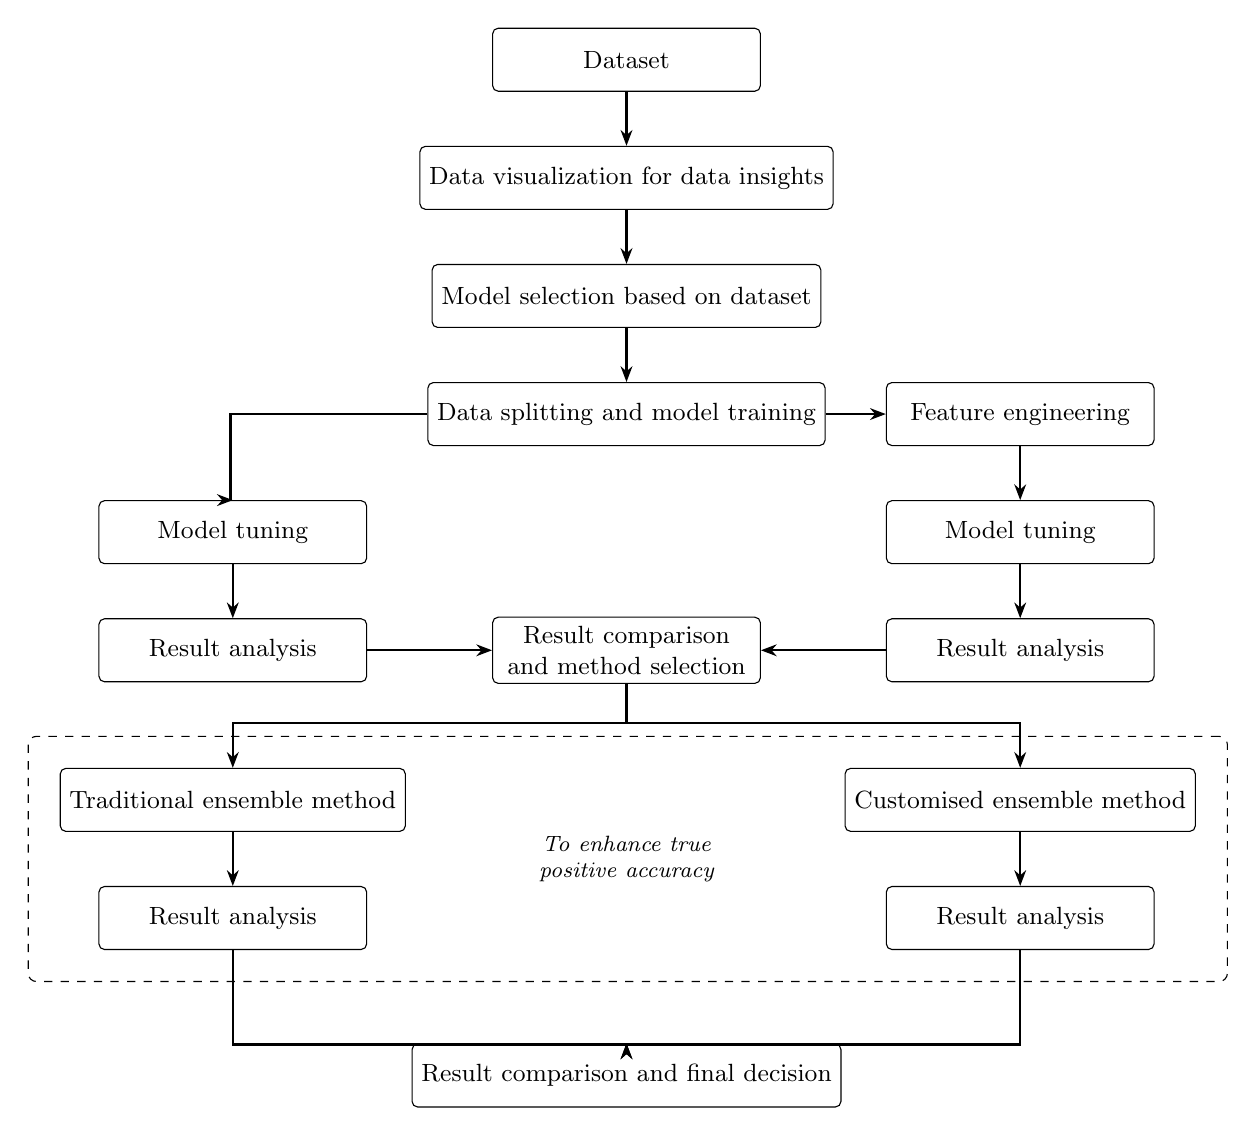
\begin{tikzpicture}[
  block/.style={draw, rounded corners=2pt, minimum width=34mm, minimum height=8mm,
                align=center, font=\small},
  arr/.style={-{Stealth[length=2mm]}, thick},
  lab/.style={font=\footnotesize\itshape, align=center}
]

% --- main vertical spine ---
\node[block] (dataset) at (0,0) {Dataset};
\node[block] (viz)     at (0,-1.5) {Data visualization for data insights};
\node[block] (modsel)  at (0,-3.0) {Model selection based on dataset};
\node[block] (split)   at (0,-4.5) {Data splitting and model training};

% --- feature-engineering branch ---
\node[block] (feat)    at (5.0,-4.5) {Feature engineering};
\node[block] (tuneL)   at (-5.0,-6.0) {Model tuning};
\node[block] (tuneR)   at (5.0,-6.0) {Model tuning};
\node[block] (raL)     at (-5.0,-7.5) {Result analysis};
\node[block] (raR)     at (5.0,-7.5) {Result analysis};
\node[block] (comp)    at (0,-7.5) {Result comparison\\and method selection};

% --- ensemble comparison stage ---
\node[block] (trad)    at (-5.0,-9.4) {Traditional ensemble method};
\node[block] (cust)    at (5.0,-9.4) {Customised ensemble method};
\node[block] (raL2)    at (-5.0,-10.9) {Result analysis};
\node[block] (raR2)    at (5.0,-10.9) {Result analysis};
\node[lab]   (note)    at (0,-10.15) {To enhance true\\positive accuracy};

\node[draw, dashed, rounded corners=3pt, inner sep=4mm,
      fit=(trad)(cust)(raL2)(raR2)(note)] (ensbox) {};

\node[block] (final)   at (0,-12.9) {Result comparison and final decision};

% --- arrows ---
\draw[arr] (dataset) -- (viz);
\draw[arr] (viz) -- (modsel);
\draw[arr] (modsel) -- (split);
\draw[arr] (split) -- (feat);
\draw[arr] (feat) -- (tuneR);
\draw[arr] (split.west) -- ++(-2.5,0) |- (tuneL.north);
\draw[arr] (tuneL) -- (raL);
\draw[arr] (tuneR) -- (raR);
\draw[arr] (raL) -- (comp);
\draw[arr] (raR) -- (comp);
\draw[arr] (comp.south) -- ++(0,-0.5) -| (trad.north);
\draw[arr] (comp.south) -- ++(0,-0.5) -| (cust.north);
\draw[arr] (trad) -- (raL2);
\draw[arr] (cust) -- (raR2);
\draw[arr] (raL2.south) |- ++(0,-1.2) -| (final.north);
\draw[arr] (raR2.south) |- ++(0,-1.2) -| (final.north);

\end{tikzpicture}
\caption{The workflow diagram of the research methodology.}
\label{fig:workflow}
\end{figure*}

As shown in Figure \ref{fig:workflow}, both workflows undergo independent model training and hyperparameter tuning, after which their results are analyzed and compared. The framework then evaluates two ensemble strategies: a conventional majority voting ensemble and a customized OR-logic ensemble designed to enhance failure detection. Comparative analysis of these approaches guides final model selection, prioritizing high failure sensitivity while maintaining operational feasibility. This systematic workflow enables rigorous evaluation of individual models, engineered features, and ensemble strategies against conventional predictive maintenance approaches.

\subsection{Data Preprocessing Pipeline}

As shown in the workflow and exemplified in Table \ref{tab:sample_data}, the AI4I 2020 Predictive Maintenance dataset comprising 10,000 instances forms the basis of model development. It includes five key operational variables—air temperature [K], process temperature [K], rotational speed [rpm], torque [Nm], and tool wear [min]—with machine failure labeled as 1 and normal operation as 0. The dataset is highly imbalanced, with only 339 failure instances (3.39\%).

\begin{table*}[htbp]
\centering
\caption{Sample dataset with the new derived features}
\label{tab:sample_data}
\resizebox{\textwidth}{!}{%
\begin{tabular}{lcccccccccccc}
\hline
\textbf{Product ID} & \textbf{Type} & \textbf{Air temp [K]} & \textbf{Process temp [K]} & \textbf{RPM} & \textbf{Torque [Nm]} & \textbf{Tool wear [min]} & \textbf{Failure} & \textbf{RelationTemp} & \textbf{Power (W)} & \textbf{WearRPM} & \textbf{ToolWearTorque} \\
\hline
M14860 & M & 298.1 & 308.6 & 1551 & 42.8 & 0 & 0 & -10.5 & 6951.952 & 0 & 0 \\
L47181 & L & 298.2 & 308.7 & 1408 & 46.3 & 3 & 0 & -10.5 & 6827.078 & 0.002131 & 0.064795 \\
L47182 & L & 298.1 & 308.5 & 1498 & 49.4 & 5 & 0 & -10.4 & 7749.791 & 0.003338 & 0.101215 \\
L47183 & L & 298.2 & 308.6 & 1433 & 39.5 & 7 & 0 & -10.4 & 5927.813 & 0.004885 & 0.177215 \\
L47184 & L & 298.2 & 308.7 & 1408 & 40.0 & 9 & 0 & -10.5 & 5898.123 & 0.006392 & 0.225000 \\
M14865 & M & 298.1 & 308.6 & 1425 & 41.9 & 11 & 0 & -10.5 & 6252.880 & 0.007719 & 0.262530 \\
L47186 & L & 298.1 & 308.6 & 1558 & 42.4 & 14 & 0 & -10.5 & 6918.063 & 0.008986 & 0.330189 \\
L47187 & L & 298.1 & 308.6 & 1527 & 40.2 & 16 & 0 & -10.5 & 6428.598 & 0.010478 & 0.398010 \\
M14868 & M & 298.3 & 308.7 & 1667 & 28.6 & 18 & 0 & -10.4 & 4992.900 & 0.010798 & 0.629371 \\
M14869 & M & 298.5 & 309.0 & 1741 & 28.0 & 21 & 0 & -10.5 & 5105.144 & 0.012062 & 0.750000 \\
\hline
\end{tabular}%
}
\end{table*}

\textcolor{blue}{No records were excluded, filtered, or removed at any stage: the dataset contains no missing values and no outlier rejection was applied, so the 10{,}000 published instances are used exactly as distributed, with preprocessing limited to the physics-informed feature construction defined in Section~\ref{sec:feature_engineering}.} Preprocessing involves data loading and exploratory analysis to assess feature distributions. Air temperature centers around 300 K, process temperature around 310 K, and tool wear exhibits a skewed distribution, while other features are approximately normal. The dataset is partitioned into training (75\%) and testing (25\%) sets using stratified sampling to preserve failure class proportions and ensure unbiased evaluation.

\subsection{Feature Engineering Approach}
\label{sec:feature_engineering}

Feature engineering plays a pivotal role in transforming raw sensor data into meaningful predictors that enhance model accuracy and interpretability. Based on correlation analysis and domain expertise in CNC thermomechanical behavior, four relationship-based features were constructed from sensor data to capture thermal stress, energy consumption, and tool degradation patterns. The correlation matrix analysis revealed that air temperature and process temperature exhibit strong positive correlation (0.88), while rotational speed and torque show strong negative correlation (-0.88). These observations motivated the derivation of physics-informed features. The engineered features are defined as follows:

\begin{equation}
\begin{split}
 \text{RelationTemperature} = \text{Air temperature [K]} - \\  \text{Process temperature [K]}   
\end{split}
\end{equation}

\begin{equation}
\text{Power [W]} = \frac{\text{Torque [Nm]} \times \text{Rotational speed [rpm]}}{9.5488}
\end{equation}

\begin{equation}
\text{WearRPM} = \frac{\text{Tool wear [min]}}{\text{Rotational speed [rpm]}}
\end{equation}

\begin{equation}
\text{ToolWearTorque} = \frac{\text{Tool wear [min]}}{\text{Torque [Nm]}}
\end{equation}

Relation Temperature captures the thermal stress gradient between ambient air and process temperature, indicating cooling system efficacy and thermal strain on machine components. Analysis revealed that failures occur more frequently when this difference falls outside the range of -12.1 K to -7.6 K. Power represents energy consumption dynamics, derived from torque and rotational speed, capturing mechanical load patterns. Machines operating within 3515.22 W to 8998.49 W showed significantly lower failure rates. WearRPM quantifies tool degradation velocity by normalizing tool wear against rotational speed, with values below 0.174 indicating optimal operational conditions. ToolWearTorque measures tool loading ratio, with threshold values below 0.26253 minimizing machine failure probability. These engineered features enable earlier identification of degradation patterns compared to raw sensor inputs alone.

\subsection{Base Classifiers}

Five supervised machine learning algorithms serve as base classifiers in the proposed ensemble framework. \textcolor{blue}{They were chosen to maximise decision-boundary diversity rather than to identify a single strongest model: because the OR-logic rule predicts a failure whenever any member does, its effectiveness depends on members that err on different instances, and our analysis shows the OR-logic advantage grows with base-learner diversity. Pairing a margin-based (SVM), bagged-tree (Random Forest), instance-based (KNN), linear (Logistic Regression), and boosted-tree (Gradient Boosting) learner provides this coverage. Neural networks were considered but not adopted: the dataset comprises independent cross-sectional records with no per-machine temporal sequences for architectures such as LSTM or TCN to exploit, and on small tabular data gradient-boosted trees have repeatedly been shown to match or exceed deep networks}~\cite{grinsztajn2022tree,shwartz2022tabular}. \textcolor{blue}{Consistent with this, a multilayer perceptron under the same protocol matched the strongest tree model's discrimination (AUC 0.977 versus 0.976) but detected fewer failures while adding tuning cost and reducing interpretability. Full configuration and results are available in the accompanying repository.\footnote{\url{https://github.com/Ashfak-Kausik/Basic-PdM-model-for-Manufacturing-Equipment}} We therefore retain these five interpretable, low-latency learners and leave sequence-aware neural models to future work.}

\subsubsection{Support Vector Machine (SVM)}

Support Vector Machine constructs optimal hyperplanes in high-dimensional feature space to separate failure and non-failure classes. The algorithm seeks to maximize the margin between classes while minimizing classification error. For a binary classification problem with training data $\{(x_i, y_i)\}$ where $x_i \in \mathbb{R}^n$ and $y_i \in \{-1, 1\}$, the SVM optimization problem is formulated as:

\begin{equation}
\min_{w,b} \frac{1}{2}\|w\|^2 + C\sum_{i=1}^{n}\xi_i
\end{equation}

subject to $y_i(w^T x_i + b) \geq 1 - \xi_i$ and $\xi_i \geq 0$, where $w$ is the weight vector, $b$ is the bias term, $C$ is the regularization parameter, and $\xi_i$ are slack variables. The kernel trick enables SVM to handle non-linearly separable data by mapping inputs to higher-dimensional spaces.

\subsubsection{Random Forest Classifier (RFC)}

Random Forest is an ensemble learning method that constructs multiple decision trees during training and outputs the mode of class predictions. Each tree is trained on a bootstrap sample of the training data, and at each node split, a random subset of features is considered. For a forest of $T$ trees, the final prediction is:

\begin{equation}
\hat{y} = \text{mode}\{h_1(x), h_2(x), ..., h_T(x)\}
\end{equation}

where $h_t(x)$ represents the prediction of the $t$-th tree. Random Forest reduces overfitting through bagging and feature randomization, providing robust predictions even with noisy data. The algorithm uses numerous decision trees to avoid overfitting and noise, resulting in robust and effective outlier handling.

\subsubsection{K-Nearest Neighbors (KNN)}

K-Nearest Neighbors is a non-parametric algorithm that classifies instances based on the majority class among their $k$ nearest neighbors in feature space. The distance metric, typically Euclidean distance, is defined as:

\begin{equation}
d(x_i, x_j) = \sqrt{\sum_{m=1}^{n}(x_{im} - x_{jm})^2}
\end{equation}

The prediction for a test instance $x$ is determined by:

\begin{equation}
\hat{y} = \text{mode}\{y_{i_1}, y_{i_2}, ..., y_{i_k}\}
\end{equation}

where $\{i_1, i_2, ..., i_k\}$ are the indices of the $k$ nearest neighbors. KNN's simplicity and effectiveness make it suitable for local pattern recognition.

\subsubsection{Logistic Regression (LR)}

Logistic Regression models the probability of binary outcomes using the logistic function. For input features $x$, the probability of failure is computed as:

\begin{equation}
P(y=1|x) = \frac{1}{1 + e^{-(w^T x + b)}}
\end{equation}

where $w$ represents feature weights and $b$ is the bias term. The model parameters are learned by minimizing the log-loss function:

\begin{equation}
L(w, b) = -\sum_{i=1}^{n}[y_i \log(\hat{y}_i) + (1-y_i)\log(1-\hat{y}_i)]
\end{equation}

Logistic Regression provides interpretable coefficients indicating feature importance.

\subsubsection{Gradient Boosting Classifier (GBC)}

Gradient Boosting constructs an ensemble of weak learners, typically decision trees, in a sequential manner where each subsequent model corrects errors made by previous models. The algorithm minimizes a loss function through gradient descent in function space:

\begin{equation}
F_m(x) = F_{m-1}(x) + \gamma_m h_m(x)
\end{equation}

where $F_m(x)$ is the ensemble prediction after $m$ iterations, $h_m(x)$ is the $m$-th weak learner, and $\gamma_m$ is the learning rate. The weak learner $h_m(x)$ is trained to predict the negative gradient of the loss function. Gradient Boosting enhances accuracy by progressively creating trees and iteratively correcting errors, particularly for difficult-to-predict situations.

\subsection{Proposed Ensemble Architecture}
The proposed ensemble framework addresses the critical limitation of traditional voting-based ensembles: their inability to prioritize failure detection sensitivity in highly imbalanced datasets. Traditional ensemble methods employ majority voting, where the final prediction is determined by the mode of individual model predictions. However, this symmetric aggregation treats false negatives (missed failures) and false positives (unnecessary inspections) as equally undesirable, failing to encode the asymmetric cost structure inherent to industrial maintenance operations.

\subsubsection{Ensemble Strategy and Design}

In CNC manufacturing environments, the cost of a false negative—resulting in undetected equipment failure, catastrophic damage, production line shutdown, and potential safety hazards—vastly exceeds the cost of a false positive, which merely triggers an unnecessary inspection. This asymmetry necessitates a classification strategy that explicitly prioritizes recall (sensitivity) over aggregate accuracy. The proposed modified ensemble method employs OR-logic classification: a machine failure is predicted if \textbf{any} constituent model detects anomalous behavior, rather than requiring consensus among models.

\subsubsection{Mathematical Formulation}

Let $f_{\text{SVM}}(x)$, $f_{\text{RF}}(x)$, $f_{\text{KNN}}(x)$, $f_{\text{LR}}(x)$, and $f_{\text{GBC}}(x)$ denote the binary predictions of the five base classifiers for input $x$, where each $f_i(x) \in \{0, 1\}$ indicates non-failure (0) or failure (1).

\textbf{Traditional Voting Ensemble:}
\begin{equation}
\hat{y}_{\text{voting}}(x) = \begin{cases} 
1 & \text{if } \sum_{i} f_i(x) \geq k \\
0 & \text{otherwise}
\end{cases}
\end{equation}

where $k$ is the voting threshold, typically set to $\lceil N/2 \rceil$ for majority voting with $N=5$ models.

\textbf{Modified OR-Logic Ensemble:}
\begin{equation}
\hat{y}_{\text{ensemble}}(x) = \max\{f_{\text{SVM}}(x), f_{\text{RF}}(x), f_{\text{KNN}}(x), f_{\text{LR}}(x), f_{\text{GBC}}(x)\}
\end{equation}

Equivalently:
\begin{equation}
\hat{y}_{\text{ensemble}}(x) = \begin{cases} 
1 & \text{if any } f_i(x) = 1 \\
0 & \text{if all } f_i(x) = 0
\end{cases}
\end{equation}

This formulation ensures that failure is predicted whenever at least one base classifier detects anomalous behavior, maximizing sensitivity at the potential cost of increased false positives. The rationale is that in predictive maintenance applications, it is preferable to investigate a potential failure that turns out to be benign rather than miss an actual failure that could lead to catastrophic consequences. \textcolor{blue}{The recall advantage of OR-logic over majority voting follows directly from this formulation. Since the OR-logic prediction is the union of the members' positive detections, its set of detected failures contains that of every individual model; its recall is therefore bounded below by the best single member and strictly exceeds it whenever different members catch different failures. Majority voting, by contrast, requires agreement from at least $\lceil N/2 \rceil$ members, so a correct minority detection is discarded whenever the remaining models miss, precisely the regime that dominates under severe class imbalance. The same union that raises recall also unions the members' false-positive rates, which is why OR-logic trades precision for sensitivity rather than obtaining a free improvement; under the asymmetric cost structure of maintenance, this is a favorable trade. This mechanism implies that the OR-logic advantage should be largest when base learners are diverse (their errors are decorrelated), a prediction we examine directly by simulation below.}

\subsubsection{Ensemble Algorithm}

The implementation of the modified ensemble method follows this procedure:
\begin{enumerate}
    \item Train each base classifier ($f_{\text{SVM}}$, $f_{\text{RF}}$, $f_{\text{KNN}}$, $f_{\text{LR}}$, $f_{\text{GBC}}$) independently on the training dataset containing both original and engineered features.
    
    \item For each test instance $x$, obtain binary predictions from all five classifiers.
    
    \item Apply OR-logic aggregation: if any classifier predicts failure ($f_i(x) = 1$), classify the instance as failure; otherwise, classify as non-failure.
    
    \item Evaluate ensemble performance using metrics appropriate for imbalanced classification: accuracy, precision, recall (true positive rate), specificity (true negative rate), F1-score, and Matthews Correlation Coefficient (\cite{chicco2020advantages}).
\end{enumerate}

The traditional voting classifier is also implemented for comparison, where failure is predicted only if the majority of classifiers (at least 3 out of 5) predict failure.

\subsubsection{Comparison of Aggregation Strategies}

The ensemble architecture integrates multiple base learners through parallel prediction pathways. Each classifier processes the same input features independently, generating binary predictions based on its learned decision boundary. The traditional voting ensemble aggregates these predictions through majority voting, while the modified ensemble employs OR-logic to maximize failure detection sensitivity. This dual evaluation enables direct comparison of symmetric versus asymmetric ensemble strategies.

The modified ensemble achieved 98.20\% overall accuracy while reducing false negatives from 48.2\% (traditional voting) to 20\%, correctly identifying 80\% of failure events. This represents a 58\% reduction in missed failures compared to traditional voting methods, while maintaining 98.8\% specificity in non-failure case identification. The ensemble's performance demonstrates that explicitly encoding operational cost asymmetry into the classification logic yields substantial improvements in failure detection sensitivity, the primary objective of predictive maintenance systems.

\subsection{Simulation Analysis of Aggregation Behavior}
\textcolor{blue}{To isolate why OR-logic outperforms majority voting independently of this particular dataset, we simulate a five-detector ensemble on a rare-positive population at 3.4\% prevalence. Each detector's per-instance errors are generated with a controllable pairwise correlation $\rho$, swept from $0$ (independent errors) to $0.8$ (highly correlated errors), and the recall of OR-logic and majority voting is averaged over many trials at each level. As shown in Figure~\ref{fig:sim_or_vs_voting}, OR-logic recall exceeds majority voting across the entire range: the gap is largest when detectors are diverse ($+0.52$ at $\rho=0$) and shrinks but never closes as their errors become correlated ($+0.37$ at $\rho=0.8$). This confirms the mechanism above, that OR-logic converts complementary, decorrelated detections into higher aggregate recall, and provides the theoretical basis for retaining diverse base learners rather than rebalancing them toward a single behavior.}

\begin{figure}[htbp]
    \centering
    
\includegraphics[width=0.7\linewidth]{fig52.png}
    \caption{\textcolor{blue}{Simulated recall of OR-logic versus majority-voting aggregation for a five-detector ensemble.}}
    \label{fig:sim_or_vs_voting}
\end{figure}

\section{Experimental Setup}

This section outlines the experimental framework adopted in this study, including the dataset characteristics, feature engineering procedures, hyperparameter settings, evaluation metrics, and computational environment. The design of the experimental setup emphasizes reproducibility and objective assessment of the proposed ensemble-based predictive maintenance framework.

\subsection{Dataset Description}

The AI4I 2020 Predictive Maintenance dataset \cite{matzka2020ai4i} from the UCI Machine Learning Repository is used as the primary benchmark for experimental evaluation. It contains 10{,}000 instances with five operational variables—air temperature, process temperature, rotational speed, torque, and tool wear—along with a binary machine failure label. Although synthetically generated, the dataset models realistic CNC operating conditions, capturing thermal behavior, mechanical loading, and tool degradation patterns. Its structured multivariate representation makes it suitable for comparative evaluation of data-driven PdM models.

Table~\ref{tab:dataset_stats} summarizes the dataset statistics. Operating parameters exhibit realistic ranges consistent with CNC environments, while failure events account for only 3.39\% of samples, reflecting real-world class imbalance. This poses a challenge for predictive models that must balance early fault detection with false alarm control.

Exploratory data analysis highlights distribution and correlation patterns (\cite{dhummad2025imperative}). Figure~\ref{fig:normal_dist} shows the distributions of operational parameters: all but tool wear are approximately normal, supporting reliable model training. Correlation analysis reveals that air temperature and process temperature are strongly positively correlated (0.88), while rotational speed and torque are strongly negatively correlated (-0.88). These insights inform the feature engineering strategy, identifying derived features that capture physically meaningful relationships in CNC operations.

\begin{table*}[htbp]
\centering
\caption{Statistical summary of the AI4I 2020 Predictive Maintenance dataset}
\label{tab:dataset_stats}
\small
\begin{tabular}{lrrrrrrrr}
\hline
\textbf{Metric} & \textbf{Count} & \textbf{Mean} & \textbf{Std} & \textbf{Min} & \textbf{25\%} & \textbf{50\%} & \textbf{75\%} & \textbf{Max} \\
\hline
UDI & 10000 & 5000.5 & 2886.9 & 1 & 2500.8 & 5000.5 & 7500.3 & 10000 \\
Air temp. [K] & 10000 & 300.0 & 2.0 & 295.3 & 298.3 & 300.1 & 301.5 & 304.5 \\
Proc. temp. [K] & 10000 & 310.0 & 1.5 & 305.7 & 308.8 & 310.1 & 311.1 & 313.8 \\
Rot. speed [rpm] & 10000 & 1538.8 & 179.3 & 1168 & 1423 & 1503 & 1612 & 2886 \\
Torque [Nm] & 10000 & 40.0 & 10.0 & 3.8 & 33.2 & 40.1 & 46.8 & 76.6 \\
Tool wear [min] & 10000 & 108.0 & 63.7 & 0 & 53 & 108 & 162 & 253 \\
Machine failure & 10000 & 0.034 & 0.181 & 0 & 0 & 0 & 0 & 1 \\
\hline
\end{tabular}
\end{table*}

\begin{figure*}[!htb]
    \centering
    
\includegraphics[width=1.5\columnwidth]{fig23.png}
    \caption{Normal distribution curves of air temperature, process temperature, rotational speed, torque, and tool wear}
    \label{fig:normal_dist}
\end{figure*}

\subsection{Hyperparameter Configuration}
\label{sec:hyperparameters}

Hyperparameter selection is critical for balancing predictive accuracy, robustness, and computational efficiency. All models were configured using empirically validated settings commonly adopted in predictive maintenance studies, with explicit consideration of nonlinearity and severe class imbalance.

Support Vector Machines (SVM) employed a radial basis function (RBF) kernel with $C = 1.0$ and kernel width determined by the \textit{scale} heuristic, $\gamma = \frac{1}{n_{\text{features}}\mathrm{Var}(X)}$. Random Forest Classifiers (RFC) were configured with 100 trees using bootstrap aggregation and feature subsampling ($\sqrt{n_{\text{features}}}$) at each split, allowing unrestricted tree depth and minimal node-splitting constraints to promote ensemble diversity. Logistic Regression (LR) utilized L2 regularization with $C = 1.0$, optimized via the \textit{lbfgs} solver with a maximum of 1000 iterations. K-Nearest Neighbors (KNN) was configured with $k = 5$ using Euclidean distance and uniform neighbor weighting, with automatic selection of the most efficient search algorithm. Gradient Boosting Machines (GBM) employed 100 boosting iterations with a learning rate of $\eta = 0.1$, tree depth limited to 3, and log-loss as the objective function to control overfitting.

\textcolor{blue}{A multilayer perceptron (two hidden layers of 64 and 32 ReLU units, L2 penalty 0.0001, early stopping) was additionally evaluated as a standalone neural baseline on the same standardised features and split; it was used for comparison only and not included in either ensemble; its results are reported in Section~\ref{sec:results_modified_individual}.} The proposed ensemble framework integrates these base learners using two aggregation strategies. A traditional hard-voting ensemble assigns equal weights to all classifiers and predicts failure when at least three out of five models agree. In contrast, the modified OR-logic ensemble predicts failure if any single base classifier detects an anomaly, effectively lowering the decision threshold to $k=1$ and prioritizing recall over precision to enhance early fault detection.

\subsection{Evaluation Metrics}

Comprehensive evaluation requires multiple metrics, particularly for imbalanced classification problems where accuracy alone can be misleading. The confusion matrix forms the foundation for all metrics, as defined in Table~\ref{tab:confusion_definition}.

\begin{table*}[htbp]
\centering
\caption{Confusion matrix structure used as the basis for all evaluation metrics.}
\label{tab:confusion_definition}
\begin{tabular}{cc|cc}
\multicolumn{2}{c}{} & \multicolumn{2}{c}{\textbf{Predicted Class}} \\
\multicolumn{2}{c|}{} & \textbf{Negative (0)} & \textbf{Positive (1)} \\
\hline
\multirow{2}{*}{\textbf{Actual Class}} & \textbf{Negative (0)} & True Negative (TN) & False Positive (FP) \\
& \textbf{Positive (1)} & False Negative (FN) & True Positive (TP) \\
\end{tabular}
\end{table*}

Based on this confusion matrix, multiple evaluation metrics were used to assess model performance, particularly under imbalanced classification settings where accuracy alone can be misleading. Accuracy indicates the proportion of correctly classified instances but does not reflect error asymmetry in failure prediction. Precision measures the reliability of positive predictions, while recall (sensitivity) evaluates the model’s ability to correctly identify actual failure events. The F1-score, as the harmonic mean of precision and recall, provides a balanced assessment when both false positives and false negatives are consequential. Specificity quantifies the correct identification of non-failure cases, helping to reduce unnecessary maintenance actions. The false negative rate was given special attention due to its direct impact on unplanned downtime and equipment failure. Collectively, these metrics offer a comprehensive evaluation framework that balances detection effectiveness with operational reliability.

\subsection{Experimental Environment}
\label{sec:experimental_environment}
All experiments were conducted under a controlled and reproducible computational environment to ensure fair model comparison. The experimental platform consisted of a 13th Gen Intel Core i5-13400F processor (16 logical cores) with 16~GB RAM, running Ubuntu Linux. The predictive maintenance framework was implemented in Python~3.10, utilizing NumPy and Pandas for numerical computation and data handling, Scikit-learn (v1.7) for model implementation and evaluation, imbalanced-learn for resampling comparisons, SHAP for explainability analysis, and Matplotlib and Seaborn for result visualization. Experiments were developed and executed using Jupyter Notebook and standalone Python scripts.

The experimental pipeline followed a standardized workflow comprising data loading, feature engineering, stratified train–test splitting (75\%–25\%) to preserve class distribution, independent model training, prediction generation, ensemble aggregation, and performance evaluation. Traditional hard voting was implemented using \texttt{VotingClassifier}, while the proposed OR-logic ensemble was realized through a custom element-wise maximum operation across classifier outputs. All experiments were executed with a fixed random seed (\texttt{random\_state=42}) to ensure reproducibility. Training times ranged from seconds for linear and instance-based models to minutes for ensemble tree-based methods, while ensemble aggregation incurred negligible computational overhead. \textcolor{blue}{To assess robustness rather than rely on a single split, all reported metrics were additionally evaluated over 30 stratified resamples (distinct random seeds); we report 95\% percentile confidence intervals across these resamples and test differences between methods using the paired Wilcoxon signed-rank test.}

\section{Results and Analysis}

This section presents comprehensive experimental results demonstrating the effectiveness of the proposed PdM framework. Results are organized to show the progression from baseline model performance on raw data, through the impact of feature engineering, to the final ensemble model performance. All findings are supported by detailed confusion matrices, performance metrics, and comparative visualizations.

\subsection{Baseline Performance on Raw Data}
The baseline evaluation establishes reference performance using raw sensor data without feature engineering or cost-sensitive learning. Due to the severe class imbalance, most models achieved high overall accuracy but exhibited poor failure detection capability. These results highlight the limitations of conventional classifiers when applied directly to imbalanced predictive maintenance datasets and motivate the need for enhanced feature representation and ensemble strategies.

\subsubsection{Individual Model Results}

Initial experiments evaluated five supervised machine learning algorithms on the original dataset containing five operational parameters: air temperature, process temperature, rotational speed, torque, and tool wear. Table \ref{tab:baseline_performance} summarizes the baseline performance metrics for individual classifiers.

\begin{table*}[htbp]
\centering
\caption{Baseline performance of individual models on raw data}
\label{tab:baseline_performance}
\begin{tabular}{lccccc}
\hline
\textbf{Model} & \textbf{Accuracy} & \textbf{Precision} & \textbf{Recall} & \textbf{F1-Score} & \textbf{Specificity} \\
\hline
SVM & 0.9720 & 0.8261 & 0.2235 & 0.3519 & 0.9983 \\
RFC & 0.9840 & 0.8571 & 0.6353 & 0.7297 & 0.9963 \\
KNN & 0.9732 & 0.7500 & 0.3176 & 0.4463 & 0.9963 \\
LR & 0.9696 & 0.7368 & 0.1647 & 0.2692 & 0.9979 \\
GBC & 0.9852 & 0.8871 & 0.6471 & 0.7483 & 0.9971 \\
\hline
\end{tabular}
\end{table*}

\textcolor{blue}{The baseline results reveal a consistent pattern across all models: while overall accuracy exceeds 96\% and specificity remains above 99.6\%, recall (failure detection sensitivity) varies dramatically. Gradient Boosting and Random Forest achieve the strongest baseline performance, with recall rates of 64.71\% and 63.53\% respectively, demonstrating their capacity to detect complex patterns in the original feature space -- GBC edges out RF as the best individual model even on raw, unengineered features. SVM exhibits the lowest recall (22.35\%), missing over three-quarters of actual failures despite maintaining high specificity. KNN and Logistic Regression achieve recall of 31.76\% and 16.47\% respectively, indicating limited effectiveness for failure detection on raw features alone.}

\subsubsection{Confusion Matrices and Performance Metrics}
Confusion matrices reveal the classification behavior across baseline and improved models, demonstrating the challenges of imbalanced failure prediction and the effectiveness of proposed solutions.

\textcolor{blue}{Models trained on original data exhibit the classic imbalanced classification problem: all achieve true negatives exceeding 2,406 of 2,415 non-failure test instances (>99.6\%) with few false positives (4--9), but show highly variable failure detection out of 85 actual failures -- true positives range from 14 (LR) to 55 (GBC) and false negatives from 30 (GBC) to 71 (LR). This confirms that standard ML models with symmetric loss functions prioritize majority class accuracy over minority class detection, fundamentally inadequate for predictive maintenance.}

Figure \ref{fig:confusion_modified} presents confusion matrices for models trained on modified data with engineered features, showing substantial detection improvements. All models maintain high true negative rates exceeding 99.5\% (TN > 2,403 of 2,415). True positive performance varies substantially: Gradient Boosting achieves the highest recall at 80.00\% (68 TP, 17 FN), closely followed by Random Forest at 77.65\% (66 TP, 19 FN), then KNN at 40.00\% (34 TP, 51 FN), SVM at 31.76\% (27 TP, 58 FN), and Logistic Regression at 22.35\% (19 TP, 66 FN). Gradient Boosting now edges out Random Forest as the strongest individual model on the modified feature set, with both tree-based ensembles substantially outperforming the linear, instance-based, and kernel approaches for this imbalanced CNC maintenance dataset.

\begin{figure*}[!htb]
    \centering
    \begin{subfigure}[b]{0.32\textwidth}
        \centering
        
\includegraphics[width=\linewidth]{fig32.png}
        \caption{Support Vector Machine}
        \label{fig:confusion_svm}
    \end{subfigure}
    \hfill
    \begin{subfigure}[b]{0.32\textwidth}
        \centering
        
\includegraphics[width=\linewidth]{fig34.png}
        \caption{Random Forest}
        \label{fig:confusion_rf}
    \end{subfigure}
    \hfill
    \begin{subfigure}[b]{0.32\textwidth}
        \centering
        
\includegraphics[width=\linewidth]{fig36.png}
        \caption{K-Nearest Neighbors}
        \label{fig:confusion_knn}
    \end{subfigure}

    \vspace{0.4cm}

    \begin{subfigure}[b]{0.32\textwidth}
        \centering
        
\includegraphics[width=\linewidth]{fig38.png}
        \caption{Logistic Regression}
        \label{fig:confusion_lr}
    \end{subfigure}
    \hfill
    \begin{subfigure}[b]{0.32\textwidth}
        \centering
        
\includegraphics[width=\linewidth]{fig40.png}
        \caption{Gradient Boosting}
        \label{fig:confusion_gbm}
    \end{subfigure}
    \hfill
    \begin{subfigure}[b]{0.32\textwidth}
        \phantom{}
    \end{subfigure}

    \caption{Confusion matrices for all five individual machine learning models on modified data with engineered features.}
    \label{fig:confusion_modified}
\end{figure*}

Figure \ref{fig:confusion_ensembles} compares traditional voting and proposed OR-logic ensembles, revealing fundamental differences in classification strategies.

\begin{figure}[!htb]
    \centering
    \begin{subfigure}[b]{0.48\textwidth}
        \centering
        
\includegraphics[width=0.7\columnwidth]{fig42.png}
        \caption{Traditional Voting Ensemble}
        \label{fig:confusion_voting}
    \end{subfigure}
    \hfill
    \begin{subfigure}[b]{0.48\textwidth}
        \centering
        
\includegraphics[width=0.7\columnwidth]{fig43.png}
        \caption{Proposed OR-Logic Ensemble}
        \label{fig:confusion_orlogic}
    \end{subfigure}
    \caption{Confusion matrices comparing traditional voting ensemble and proposed OR-logic ensemble on modified data}
    \label{fig:confusion_ensembles}
\end{figure}

Traditional voting achieves near-perfect non-failure identification (2,413 TN, 2 FP) but detects only 44 of 85 failures (51.76\% recall), missing 41. OR-logic achieves 2,387 TN (98.84\% specificity) with 28 FP (1.16\% false alarm rate) while identifying 68 of 85 failures (80.00\% recall), missing only 17. By tolerating 26 additional false positives, OR-logic identifies 24 additional true failures -- a 54.5\% relative improvement in recall over voting. Operationally, accepting 26 additional inspections prevents 24 additional catastrophic failures, favorable given asymmetric costs where undetected failures exceed inspection costs by orders of magnitude.

\begin{table*}[htbp]
\centering
\caption{Detailed performance metrics comparing individual models and ensemble approaches}
\label{tab:detailed_metrics}
\begin{tabular}{lccccc}
\hline
\textbf{Metric} & \textbf{SVM} & \textbf{RFC} & \textbf{GBC} & \textbf{Voting} & \textbf{OR-Logic} \\
\hline
\textbf{Overall Performance} & & & & & \\
\quad Accuracy & 97.6\% & 99.0\% & 98.9\% & 98.3\% & \textbf{98.2\%} \\
\quad Precision & 90.0\% & 91.7\% & 87.2\% & 95.7\% & \textbf{70.8\%} \\
\quad Recall & 31.8\% & 77.6\% & 80.0\% & 51.8\% & \textbf{80.0\%} \\
\quad F1-Score & 47.0\% & 84.1\% & 83.4\% & 67.2\% & \textbf{75.1\%} \\
\hline
\textbf{Confusion Matrix Elements} & & & & & \\
\quad True Positives & 27 & 66 & 68 & 44 & \textbf{68} \\
\quad False Negatives & 58 & 19 & 17 & 41 & \textbf{17} \\
\quad True Negatives & 2,412 & 2,409 & 2,405 & 2,413 & \textbf{2,387} \\
\quad False Positives & 3 & 6 & 10 & 2 & \textbf{28} \\
\hline
\textbf{Error Rates} & & & & & \\
\quad False Negative Rate & 68.24\% & 22.35\% & 20.00\% & 48.24\% & \textbf{20.00\%} \\
\quad False Positive Rate & 0.12\% & 0.25\% & 0.41\% & 0.08\% & \textbf{1.16\%} \\
\hline
\end{tabular}
\end{table*}

Table \ref{tab:detailed_metrics} shows that OR-logic ties the best individual model, GBC, for the lowest false negative rate on this split -- both at 20.00\% (17 of 85 failures missed) -- while traditional voting misses 48.24\% of failures. This represents a 58.5\% relative reduction in missed failures versus traditional voting. Against the best individual model, OR-logic is exactly tied on this single SEED=42 split rather than superior to it; its advantage over GBC is a cross-seed effect, with a +3.8 percentage-point mean recall gain averaged over 30 stratified resamples (paired Wilcoxon signed-rank test, $p<0.001$). OR-logic's false positive rate (1.16\%) is higher than GBC's (0.41\%), reflecting the deliberate trade-off of tolerating more false alarms in exchange for matching GBC's failure-detection sensitivity via a simpler, more transparent union rule. This demonstrates OR-logic aggregation's effectiveness in leveraging complementary detection patterns across diverse base learners, directly aligning with predictive maintenance objectives: minimize missed failures while maintaining manageable false alarms.

\subsection{Feature Engineering and Data Modification}
Feature engineering transforms raw sensor measurements into physics-informed variables that capture critical degradation mechanisms. Four engineered features were created: Relation Temperature (thermal gradient), Power (mechanical energy), WearRPM (normalized wear rate), and ToolWearTorque (wear-torque interaction). Each is derived directly from the recorded operational variables using the relationships defined in Section~\ref{sec:feature_engineering}, and the resulting nine-feature representation is used unchanged across all models to ensure comparability. Detailed performance analysis and impact assessment are presented in Section~\ref{sec:ensemble_performance}.

\subsection{Impact of Feature Engineering and Data Modification}

The impact of feature engineering is evaluated by comparing model performance before and after feature augmentation and data modification. Physics-informed features significantly improve class separability, leading to notable gains in recall and F1-score across all models. These improvements demonstrate that embedding domain knowledge into the feature space enhances failure sensitivity without disproportionately increasing false positives, thereby strengthening model reliability for real-world predictive maintenance applications.

\subsubsection{Feature Engineering Overview and Validation}

Feature engineering transformed raw sensor measurements into physics-informed variables capturing critical degradation mechanisms. Four engineered features were developed based on domain knowledge of CNC operations:

\begin{itemize}
    \item \textbf{Relation Temperature}: Thermal gradient between process and air temperature, capturing thermal stress conditions
    \item \textbf{Power}: Mechanical power derived from torque and rotational speed, indicating energy consumption patterns
    \item \textbf{WearRPM}: Normalized tool wear rate accounting for operational speed
    \item \textbf{ToolWearTorque}: Interaction term capturing the combined effect of wear and mechanical loading
\end{itemize}

Exploratory analysis validates the discriminative power of these engineered features. Figure~\ref{fig:scatter_engineered} presents scatter plots illustrating relationships between engineered features and machine failure. Relation Temperature shows that failures occur outside optimal thermal gradients, Power highlights failures at extreme energy loads, and both WearRPM and ToolWearTorque exhibit threshold behaviors corresponding to increased failure risk. These patterns confirm that engineered features provide meaningful predictive indicators.

\begin{figure*}[!htb]
    \centering
    
\includegraphics[width=1.5\columnwidth]{fig51.png}
    \caption{Scatter plots showing relationship between engineered features and machine failure}
    \label{fig:scatter_engineered}
\end{figure*}

Comparative analysis of models trained on original versus modified features demonstrates the substantial impact of feature engineering. Table~\ref{tab:feature_comparison} summarizes the improvement in accuracy and recall. \textcolor{blue}{Engineered features consistently enhance predictive performance, particularly recall for failure detection. GBC and RFC achieve the largest absolute recall gains, while SVM, KNN, and LR -- starting from a much lower baseline recall -- also improve meaningfully, though by smaller absolute percentage-point margins, validating the effectiveness of physics-informed feature engineering in enabling more robust failure prediction.}

\begin{table}[htbp]
\centering
\caption{Performance comparison: original features vs. modified features}
\label{tab:feature_comparison}
\small
\begin{tabular}{lcccc}
\hline
\textbf{Model} & \multicolumn{2}{c}{\textbf{Original Features}} & \multicolumn{2}{c}{\textbf{Modified Features}} \\
 & \textbf{Accuracy} & \textbf{Recall} & \textbf{Accuracy} & \textbf{Recall} \\
\hline
SVM & 0.9720 & 0.2235 & 0.9756 & 0.3176 \\
RFC & 0.9840 & 0.6353 & 0.9900 & 0.7765 \\
KNN & 0.9732 & 0.3176 & 0.9760 & 0.4000 \\
LR & 0.9696 & 0.1647 & 0.9688 & 0.2235 \\
GBC & 0.9852 & 0.6471 & 0.9892 & 0.8000 \\
\hline
\end{tabular}
\end{table}

\subsubsection{Individual Model Results on Modified Data}
\label{sec:results_modified_individual}

Following feature engineering, models were retrained on the augmented dataset containing nine features: five original parameters plus four engineered features. \textcolor{blue}{Feature engineering yields consistent recall improvements across all models. GBC achieves the largest absolute gain, increasing recall from 64.71\% to 80.00\% (+15.29pp) while maintaining precision of 87.18\% and overall accuracy of 98.92\%, making it the strongest individual model on the modified feature set. RFC follows closely, improving from 63.53\% to 77.65\% recall (+14.12pp) with accuracy of 99.00\%. Models with weaker baseline performance also improve: SVM's recall rises from 22.35\% to 31.76\% (+9.41pp), KNN from 31.76\% to 40.00\% (+8.24pp), and LR from 16.47\% to 22.35\% (+5.88pp). These consistent improvements validate that physics-informed feature engineering enhances the discriminative capacity of the feature space, enabling more effective failure pattern recognition.}

\textcolor{blue}{To substantiate the choice of tree-based learners over neural approaches, a multilayer perceptron (MLP) was evaluated under the identical pipeline and split as a standalone comparison (Table~\ref{tab:mlp}). The MLP matches GBC on AUC but detects far fewer failures at the default threshold. It attains discrimination on par with the strongest tree model, GBC (AUC 0.977 versus 0.976), confirming that its underlying ranking ability is comparable. At the default decision threshold, however, it detects substantially fewer failures (recall 0.494 versus 0.800), and it offers no advantage while requiring additional tuning and yielding less interpretable predictors. This supports retaining the compact, interpretable tree learners for this task.}

\begin{table}[htbp]
\centering
\caption{\textcolor{blue}{Feed-forward neural baseline (MLP) versus the strongest individual model (GBC) on the modified data, single seed-42 split.}}
\label{tab:mlp}
\begin{tabular}{lccc}
\hline
Model & Recall & Precision & AUC \\
\hline
MLP & 0.494 & 0.792 & 0.977 \\
GBC (best individual) & 0.800 & 0.872 & 0.976 \\
\hline
\end{tabular}
\end{table}


Figure \ref{fig:correlation_original} illustrates the correlation structure of the original CNC machine dataset prior to feature engineering, highlighting baseline relationships among raw process variables and machine failure. This figure serves as a reference point for assessing how engineered features reshape feature interactions and improve model discrimination in subsequent analyses.

\begin{figure*}[!htb]
    \centering
    
\includegraphics[width=1.5\columnwidth]{fig30.png}
    \caption{Correlation matrix of the original CNC machine dataset prior to feature engineering}
    \label{fig:correlation_original}
\end{figure*}

\subsubsection{Performance Improvement Analysis}

Table \ref{tab:improvement_analysis} quantifies the impact of feature engineering by comparing performance metrics before and after data modification.

\begin{table*}[htbp]
\centering
\caption{Performance improvement analysis: raw data vs. modified data}
\label{tab:improvement_analysis}
\small
\begin{tabular}{lcccccc}
\hline
\textbf{Model} & \multicolumn{2}{c}{\textbf{Accuracy}} & \multicolumn{2}{c}{\textbf{Recall}} & \multicolumn{2}{c}{\textbf{Improvement}} \\
 & \textbf{Raw} & \textbf{Modified} & \textbf{Raw} & \textbf{Modified} & \textbf{Acc. (pp)} & \textbf{Recall (pp)} \\
\hline
SVM & 0.9720 & 0.9756 & 0.2235 & 0.3176 & +0.36 & +9.41 \\
RFC & 0.9840 & 0.9900 & 0.6353 & 0.7765 & +0.60 & +14.12 \\
KNN & 0.9732 & 0.9760 & 0.3176 & 0.4000 & +0.28 & +8.24 \\
LR & 0.9696 & 0.9688 & 0.1647 & 0.2235 & -0.08 & +5.88 \\
GBC & 0.9852 & 0.9892 & 0.6471 & 0.8000 & +0.40 & +15.29 \\
\hline
\end{tabular}
\end{table*}

\textcolor{blue}{The improvement analysis reveals a more nuanced picture than a uniform gain across all models. Four of the five models show modest accuracy improvements, from +0.28 to +0.60 percentage points; LR is the exception, showing a negligible accuracy decrease of -0.08 percentage points, effectively unchanged. All five models show consistent, and in most cases substantial, gains in recall, ranging from +5.88 percentage points for LR to +15.29 percentage points for GBC. Notably, GBC -- already the strongest baseline performer -- achieves the single largest absolute recall gain from feature engineering, followed closely by RFC (+14.12pp); SVM (+9.41pp), KNN (+8.24pp), and LR (+5.88pp), whose baseline recall was much lower, see smaller absolute point gains despite having access to the same engineered features. These recall gains are achieved without a general loss of specificity, as all models maintain true negative rates at or above 99.5\%, keeping false alarms in check. Precision improves for three of the five models (SVM, RFC, KNN); LR and GBC show a modest precision decrease (LR: 73.68\%$\to$61.29\%; GBC: 88.71\%$\to$87.18\%) as the modified feature set shifts their decision boundary toward higher recall, a reasonable trade-off given the recall-first objective of this application. Overall, these results validate that domain-informed feature engineering -- capturing thermal stress relationships, power dynamics, and degradation patterns -- substantially enhances failure detection performance without sacrificing operational feasibility.}

\subsubsection{Correlation Structure and Feature Validation}

\text{blue}{Before assessing predictive influence, the correlation structure of the augmented feature set is examined to verify that the engineered features are physically consistent and contribute information beyond their constituent variables.}

\begin{figure*}[!htb]
    \centering
    
\includegraphics[width=1.5\columnwidth]{fig31.png}
    \caption{Correlation matrix of original and engineered features}
    \label{fig:correlation_heatmap}
\end{figure*}

Figure \ref{fig:correlation_heatmap} presents the correlation structure among all features in the augmented dataset, revealing strong interdependencies between engineered features and their constituent parameters while confirming that engineered features introduce complementary discriminative information. Notable correlations include the strong positive relationship between Torque and Power (0.98), Tool wear and WearRPM (0.98), and the expected negative correlation between Rotational speed and Torque (-0.88), validating the physical consistency of the feature engineering approach. Importantly, none of the engineered features is fully determined by a single raw variable, confirming that each contributes complementary information rather than duplicating an existing measurement; their predictive influence is quantified in Section~\ref{sec:interpretability}.

The scatter plots in Figure \ref{fig:scatter_engineered} demonstrate clear separation patterns between failure and non-failure classes along engineered feature dimensions. Relation Temperature shows clustering of failures outside the optimal thermal range (-12.1 to -7.6 K). Power exhibits bimodal failure distribution at extreme values. WearRPM and ToolWearTorque display threshold behavior, with failure probability increasing sharply beyond critical values (0.174 and 0.263 respectively). These visualizations provide interpretable evidence that engineered features capture meaningful degradation signatures.

\subsubsection{Feature Importance and Interpretability}
\label{sec:interpretability}
\textcolor{blue}{Although the ensemble does not yield a closed-form analytical expression, its predictions remain interpretable and usable in engineering practice. Using SHAP (SHapley Additive exPlanations) on the tree-based models, we quantified each feature's contribution to individual predictions. SHAP is used in preference to impurity-based (Gini) importance, which is known to be biased toward high-cardinality and strongly correlated predictors; a material concern here given the strong correlations between the engineered features and their constituent variables reported above.The engineered features rank among the most influential predictors, alongside rather than replacing the raw sensor signals: for Random Forest the thermal-gradient feature (RelationTemperature) is the single most important variable, while for Gradient Boosting rotational speed leads with RelationTemperature and WearRPM close behind. This confirms that physics-informed feature construction adds discriminative signal complementary to the raw inputs. Practically, these attributions give operators a transparent view of which measurable quantities drive a failure alert, and the engineered features themselves carry direct physical meaning (thermal stress, mechanical power, and wear-to-load ratios), providing actionable, physically grounded decision support despite the absence of an explicit predictive formula.}

\begin{figure*}[!htb]
    \centering
    
\includegraphics[width=1.5\columnwidth]{shap_gbc.png}
    \caption{\textcolor{blue}{SHAP analysis for the Gradient Boosting model on the modified feature set. Left: per-instance SHAP values (beeswarm); right: mean absolute SHAP ranking, with engineered features marked by an asterisk.}}
    \label{fig:shap_gbc}
\end{figure*}

\textcolor{blue}{As illustrated in Figure~\ref{fig:shap_gbc}, the mean absolute SHAP ranking places three of the four engineered features, RelationTemperature, WearRPM, and Power, among the most influential predictors, interleaved with the raw rotational-speed and tool-wear signals rather than displacing them. The beeswarm panel further shows the direction of these effects: high WearRPM and high RelationTemperature values push the model output strongly toward a failure prediction, consistent with the physical intuition that elevated normalized wear and abnormal thermal gradients precede machine failure. These attributions give the authors, and by extension a maintenance operator, a transparent and physically coherent account of why a given instance is flagged, which is precisely the interpretability that a closed-form model would otherwise be expected to provide.}

\subsection{Comparison with Automatic Feature Extraction}
\textcolor{blue}{To assess whether the physics-informed features provide an advantage over generic feature construction, we compared the four engineered features (added to the five raw sensors) against an automatic tabular baseline: a degree-two polynomial expansion of the raw sensors including pairwise interactions, which produces 20 generated features. Both sets were evaluated under the identical pipeline, split, and models. The physics-informed set outperformed the larger automatic set on the failure-detection metrics (recall and AUC) for both the OR-logic ensemble and the strongest individual model, GBC (Table~\ref{tab:autofeat}), despite using roughly five times fewer generated features. For the OR-logic ensemble the automatic features were marginally higher on precision and specificity, so the engineered features are not uniformly superior; rather, they improve the metrics that matter most for this recall-first task while remaining substantially more interpretable, since a threshold on RelationTemperature carries a direct physical meaning that an automatically generated product term does not. Dedicated time-series extractors such as TSFresh and wavelet transforms were not applicable here: the AI4I 2020 data are independent cross-sectional records with no per-machine timestamp or identifier linking observations over time, so no temporal signal exists for such methods to extract.}

\begin{table*}[htbp]
\centering
\caption{\textcolor{blue}{Physics-informed engineered features versus an automatic degree-two polynomial expansion (20 generated features)}}
\label{tab:autofeat}
\begin{tabular}{llcccc}
\hline
Model & Feature set & Recall & Precision & Specificity & AUC \\
\hline
OR-Logic & Engineered & \textbf{0.800} & 0.708 & 0.988 & \textbf{0.898} \\
OR-Logic & Automatic (poly, 20) & 0.776 & \textbf{0.742} & \textbf{0.990} & 0.885 \\
GBC & Engineered & \textbf{0.800} & \textbf{0.872} & 0.996 & \textbf{0.976} \\
GBC & Automatic (poly, 20) & 0.741 & 0.863 & 0.996 & 0.966 \\
\hline
\end{tabular}
\end{table*}

\subsection{Proposed Ensemble Model Performance}
\label{sec:ensemble_performance}

The proposed ensemble model is evaluated to assess its effectiveness in addressing failure detection under severe class imbalance. Performance is analyzed in comparison with traditional voting ensembles to highlight the impact of cost-sensitive OR-logic aggregation. Results demonstrate that the proposed framework substantially improves recall and failure sensitivity while maintaining acceptable precision and specificity for industrial deployment.


\subsubsection{Ensemble Results on Raw Data}

To establish a comprehensive baseline, both traditional voting ensemble and the proposed OR-logic ensemble were evaluated on raw data (without engineered features). Table \ref{tab:ensemble_raw} presents the results.

\begin{table*}[htbp]
\centering
\caption{Ensemble performance on raw data}
\label{tab:ensemble_raw}
\begin{tabular}{lccccc}
\hline
\textbf{Ensemble Method} & \textbf{Accuracy} & \textbf{Precision} & \textbf{Recall} & \textbf{F1-Score} & \textbf{Specificity} \\
\hline
Traditional Voting & 0.9752 & 0.8485 & 0.3294 & 0.4746 & 0.9979 \\
Proposed OR-Logic & 0.9824 & 0.7531 & 0.7176 & 0.7349 & 0.9917 \\
\hline
\end{tabular}
\end{table*}

\textcolor{blue}{Even on raw data, the OR-logic ensemble demonstrates its core advantage: substantially higher recall (71.76\% vs.\ 32.94\%, a +38.8 percentage-point gain) than traditional voting, at the cost of reduced precision (75.31\% vs.\ 84.85\%, a -9.5 percentage-point decrease). Notably, OR-logic's overall accuracy is not traded away here -- it is marginally higher than voting's (98.24\% vs.\ 97.52\%). This trade-off aligns precisely with predictive maintenance priorities, where detecting failures is paramount and false alarms are operationally manageable.}

\subsubsection{Ensemble Results on Modified Data}

The proposed ensemble framework achieves optimal performance when combining the OR-logic aggregation strategy with engineered features. Table \ref{tab:ensemble_modified} presents comprehensive results.

\begin{table*}[htbp]
\centering
\caption{Ensemble performance on modified data (final results)}
\label{tab:ensemble_modified}
\begin{tabular}{lccccccc}
\hline
\textbf{Method} & \textbf{Acc.} & \textbf{Prec.} & \textbf{Recall} & \textbf{F1} & \textbf{Spec.} & \textbf{MCC} & \textbf{FN Rate} \\
\hline
Traditional Voting & 0.9828 & 0.9565 & 0.5176 & 0.6718 & 0.9992 & 0.6969 & 0.4824 \\
Proposed OR-Logic & 0.9820 & 0.7083 & 0.8000 & 0.7514 & 0.9884 & 0.7436 & 0.2000 \\
\hline
\textbf{Best Individual (GBC)} & 0.9892 & 0.8718 & 0.8000 & 0.8344 & 0.9959 & 0.8296 & 0.2000 \\
\hline
\end{tabular}
\end{table*}

\textcolor{blue}{The proposed OR-logic ensemble demonstrates a clear single-split advantage over traditional voting when applied to the modified dataset with engineered features. Overall accuracy is comparable between the two ensemble strategies (98.20\% for OR-logic vs.\ 98.28\% for voting), while OR-logic substantially improves recall to 80.00\%, correctly identifying 68 of 85 failure instances, compared to only 51.76\% (44/85) for traditional voting -- a 28.24 percentage-point absolute improvement. This directly translates into a reduction in false negative rate from 48.24\% under traditional voting to 20.00\% with OR-logic, a 58.5\% relative reduction in missed failures.}

\textcolor{blue}{Despite prioritizing failure detection, the OR-logic ensemble maintains high specificity at 98.84\%, resulting in 28 false alarms among 2,415 non-failure instances. The Matthews Correlation Coefficient of 0.744 indicates strong overall classification quality under severe class imbalance, while the F1-score of 0.751 reflects the trade-off between precision and recall implied by prioritizing recall.}

\textcolor{blue}{On this single SEED=42 split, however, OR-logic does not outperform the best individual model, GBC: the two are exactly tied on recall (80.00\%, 68/85 failures each) and false negative rate (20.00\%), and GBC in fact achieves higher accuracy (98.92\% vs.\ 98.20\%), precision (87.18\% vs.\ 70.83\%), F1-score (0.834 vs.\ 0.751), specificity (99.59\% vs.\ 98.84\%), and MCC (0.830 vs.\ 0.744) than OR-logic on this split. The ensemble's advantage over the best individual model therefore does not appear on this split at all; it emerges only across repeated partitions, where OR-logic's mean recall exceeds GBC's by +3.8 percentage points over 30 stratified resamples (paired Wilcoxon signed-rank test, $p<0.001$, $n=30$ seeds); a modest but statistically consistent cross-seed advantage. We report both results plainly, tied on this split, a small but real edge across seeds, rather than overstating a single-split tie as a win.}

\subsubsection{Statistical Robustness}
\textcolor{blue}{To quantify the reliability of the reported improvements, every metric was evaluated over 30 stratified resamples. Table~\ref{tab:stability} reports the mean and 95\% confidence interval for the key metrics of the two ensembles and the strongest individual model, and Figure~\ref{fig:recall_forest} shows the recall of all methods with these intervals. OR-logic and traditional voting intervals do not overlap; OR-logic and the best individual model (GBC) overlap at the margins but differ significantly under a paired test. The separation between OR-logic and traditional voting is unambiguous: their recall confidence intervals do not overlap. A paired Wilcoxon signed-rank test confirms this, with OR-logic exceeding traditional voting by a mean of 30.8 percentage points in recall ($p \approx 1.7\times10^{-6}$, $n=30$). Against the strongest individual model (GBC), the paired test shows OR-logic higher in recall in all 30 resamples, by a smaller mean margin of 3.8 percentage points ($p \approx 2.5\times10^{-6}$); consistent with the single-split tie reported earlier, this confirms the advantage over the best individual model is real but modest, whereas the advantage over conventional voting is large. These results establish that the reported gains are statistically significant and not artifacts of a particular train--test partition.}

\begin{table*}[htbp]
\centering
\caption{Recall, specificity, and MCC over 30 stratified resamples (mean with 95\% confidence interval).}
\label{tab:stability}
\begin{tabular}{lccc}
\hline
Method & Recall & Specificity & MCC \\
\hline
Traditional Voting & 0.469 [0.382, 0.568] & 0.999 [0.998, 1.000] & 0.63 [0.55, 0.71] \\
GBC (best individual) & 0.739 [0.661, 0.827] & 0.996 [0.993, 0.998] & 0.81 [0.75, 0.86] \\
OR-Logic (proposed) & 0.776 [0.703, 0.839] & 0.991 [0.987, 0.994] & 0.74 [0.68, 0.79] \\
\hline
\end{tabular}
\end{table*}

\begin{figure}[htbp]
    \centering
    
\includegraphics[width=0.8\linewidth]{recall_forest.png}
    \caption{\textcolor{blue}{Per-method recall over 30 stratified resamples}}
    \label{fig:recall_forest}
\end{figure}

\textcolor{blue}{To confirm that OR-logic aggregation is preferable to standard imbalance remedies rather than a substitute for them, we also evaluated SMOTE, cost-sensitive class weighting, and random undersampling within the same pipeline. Each raised raw recall to 0.95--0.98 but sharply degraded precision (to 0.12--0.16) and specificity (to 0.75--0.83) for the OR-logic ensemble, because its false-positive rate is bounded below by the union of its five members' rates, so any per-model rebalancing degrades every member and the union compounds all five. Leaving the base learners unbalanced is therefore the appropriate choice for a union ensemble as summarized in Table~\ref{tab:imbalance}}

\begin{table*}[htbp]
\centering
\caption{\textcolor{blue}{Imbalance-handling strategies applied within the pipeline (training fold only) for the OR-logic ensemble and the strongest individual model (GBC), against the unbalanced locked configuration. Every rebalancing strategy raises recall but sharply degrades precision and specificity for the union ensemble. GBC's class-weight row equals its baseline because \texttt{GradientBoostingClassifier} has no class-weight parameter.}}
\label{tab:imbalance}
\begin{tabular}{llccccc}
\hline
Strategy & Model & Recall & Precision & Specificity & F1 & MCC \\
\hline
None (locked)        & OR-Logic & 0.800 & 0.708 & 0.988 & 0.751 & 0.744 \\
SMOTE                & OR-Logic & 0.965 & 0.155 & 0.815 & 0.267 & 0.346 \\
Class-weighting      & OR-Logic & 0.953 & 0.162 & 0.827 & 0.277 & 0.354 \\
Undersampling        & OR-Logic & 0.976 & 0.122 & 0.753 & 0.217 & 0.297 \\
\hline
None (locked)        & GBC & 0.800 & 0.872 & 0.996 & 0.834 & 0.830 \\
SMOTE                & GBC & 0.906 & 0.348 & 0.940 & 0.503 & 0.540 \\
Class-weighting      & GBC & 0.800 & 0.872 & 0.996 & 0.834 & 0.830 \\
Undersampling        & GBC & 0.929 & 0.294 & 0.921 & 0.446 & 0.498 \\
\hline
\end{tabular}
\end{table*}

\subsubsection{Computational Cost}
\textcolor{blue}{Because predictive maintenance must run within tight industrial cycle times, we measured the training and inference cost of every model and of the proposed ensemble on the environment described in Section~\ref{sec:experimental_environment}. Table~\ref{tab:cost} reports per-sample inference latency and serialized model size. Inference is sub-millisecond per sample for every component: the OR-logic ensemble, whose cost is the sum of its five members, requires approximately 38~$\mu$s per sample and about 2.9~MB of memory, while the strongest individual model (GBC) requires roughly 0.7~$\mu$s and 137~KB. The ensemble is therefore more expensive than any single model by construction, yet its absolute cost remains negligible: at tens of microseconds per sample it processes tens of thousands of parts per second on a commodity desktop CPU, far exceeding the throughput of any physical CNC line and well within real-time and edge-deployment constraints without specialized accelerators. The nearest-neighbour classifier dominates the ensemble's latency, so if stricter budgets arise it is the natural candidate for optimization or removal.}

\begin{table}[htbp]
\centering
\caption{\textcolor{blue}{Training time, per-sample inference latency, and serialized model size, measured on the environment of Section~\ref{sec:experimental_environment}. The OR-logic ensemble cost is the sum of its five base learners.}}
\label{tab:cost}
\resizebox{\columnwidth}{!}{%
\begin{tabular}{lccc}
\hline
Model & Train time (s) & Inference ($\mu$s/sample) & Size (KB) \\
\hline
SVM      & 0.440 & 10.95 & 48.2 \\
RFC      & 0.928 & 4.03  & 1{,}575.6 \\
KNN      & 0.006 & 21.56 & 1{,}218.2 \\
LR       & 0.015 & 0.47  & 2.0 \\
GBC      & 1.158 & 0.7   & 137 \\
\hline
OR-Logic (ensemble) & 2.548 & 38 & 2{,}900 \\
\hline
\end{tabular}%
}
\end{table}

\subsubsection{Performance Visualization and Comparative Analysis}

Receiver Operating Characteristic (ROC) curves were generated to assess model discrimination capability across varying decision thresholds. Figure \ref{fig:roc_curves} presents the ROC curves for all five models on the modified dataset.

\begin{figure*}[!htb]
    \centering
    \begin{subfigure}[b]{0.32\textwidth}
        \centering
        
\includegraphics[width=\linewidth]{fig33.png}
        \caption{Support Vector Machine}
        \label{fig:roc_svm}
    \end{subfigure}
    \hfill
    \begin{subfigure}[b]{0.32\textwidth}
        \centering
        
\includegraphics[width=\linewidth]{fig35.png}
        \caption{Random Forest}
        \label{fig:roc_rfc}
    \end{subfigure}
    \hfill
    \begin{subfigure}[b]{0.32\textwidth}
        \centering
        
\includegraphics[width=\linewidth]{fig37.png}
        \caption{K-Nearest Neighbors}
        \label{fig:roc_knn}
    \end{subfigure}

    \vspace{0.4cm}

    \begin{subfigure}[b]{0.32\textwidth}
        \centering
        
\includegraphics[width=\linewidth]{fig39.png}
        \caption{Logistic Regression}
        \label{fig:roc_lr}
    \end{subfigure}
    \hfill
    \begin{subfigure}[b]{0.32\textwidth}
        \centering
        
\includegraphics[width=\linewidth]{fig41.png}
        \caption{Gradient Boosting}
        \label{fig:roc_gbc}
    \end{subfigure}
    \hfill
    \begin{subfigure}[b]{0.32\textwidth}
        \phantom{}
    \end{subfigure}

    \caption{ROC curves for all five machine learning models on modified data with engineered features.}
    \label{fig:roc_curves}
\end{figure*}

Tree-based ensemble methods demonstrate the strongest discriminative capacity, with RFC (AUC = 0.983) and GBC (AUC = 0.976) achieving the highest scores. SVM performs comparably well despite its low recall, with AUC = 0.973, indicating strong ranking ability that is not reflected in its default-threshold recall. LR achieves AUC = 0.904, while KNN exhibits the weakest ranking performance at AUC = 0.891. These results validate that feature engineering combined with ensemble strategies effectively enhances class separability under severe class imbalance, though AUC alone does not capture the recall differences that motivate the OR-logic ensemble's design.

Table \ref{tab:final_comparison} summarizes the complete performance evolution from baseline models through feature engineering to the final ensemble architecture.

\begin{table*}[htbp]
\centering
\caption{Complete performance comparison: baseline to final ensemble}
\label{tab:final_comparison}
\small
\begin{tabular}{lcccc}
\hline
\textbf{Approach} & \textbf{Accuracy} & \textbf{Recall} & \textbf{FN Rate} & \textbf{Improvement} \\
\hline
Best Baseline (GBC, raw) & 98.52\% & 64.71\% & 35.29\% & --- \\
Best Individual (GBC, modified) & 98.92\% & 80.00\% & 20.00\% & +15.3pp recall \\
Traditional Voting (modified) & 98.28\% & 51.76\% & 48.24\% & -28.2pp recall \\
\textbf{Proposed Ensemble (modified)} & \textbf{98.20\%} & \textbf{80.00\%} & \textbf{20.00\%} & \textbf{+28.2pp recall} \\
\hline
\textbf{vs. Baseline} & -0.32pp & +15.3pp & -15.3pp & --- \\
\textbf{vs. Best Individual} & -0.72pp & +0.0pp$^{*}$ & +0.0pp$^{*}$ & --- \\
\textbf{vs. Traditional Voting} & -0.08pp & +28.2pp & -28.2pp & --- \\
\hline
\end{tabular}
\end{table*}

\textcolor{blue}{$^{*}$OR-logic and GBC are exactly tied on recall (0.800 each) and FN rate on this single SEED=42 split; across 30 stratified resamples, OR-logic's mean recall exceeds GBC's by +3.8 percentage points (paired Wilcoxon signed-rank test, $p<0.001$, $n=30$ seeds).}

\textcolor{blue}{The proposed OR-logic ensemble achieves a +15.3 percentage-point recall improvement over the best raw baseline (GBC, 64.71\%$\to$80.00\%), essentially at parity on accuracy (-0.32pp). It is exactly tied with the best individual model on this split (GBC, modified: 80.00\% recall each); OR-logic's advantage over GBC only emerges as a +3.8 percentage-point mean recall gain across 30 resampled seeds (paired Wilcoxon signed-rank test, $p<0.001$), a real but modest cross-seed effect rather than a dramatic single-split one. OR-logic improves recall by +28.2 percentage points over traditional voting (51.76\%$\to$80.00\%), with a corresponding 28.24 percentage-point (58.5\% relative) reduction in false negative rate. These results demonstrate that physics-informed feature engineering combined with OR-logic ensemble aggregation effectively addresses failure detection challenges in imbalanced predictive maintenance datasets, with the ensemble's edge over the single best model reported honestly as a modest, statistically consistent cross-seed effect rather than a single-split win.}

\section{Discussion}\label{sec:discussion}

The experimental results demonstrate that the proposed OR-logic ensemble framework achieves substantial improvements in predictive maintenance performance through three complementary mechanisms. Physics-informed feature engineering transforms raw sensor measurements into domain-enriched representations that explicitly capture thermal stress gradients (Relation Temperature), energy consumption (Power), and tool degradation patterns (WearRPM, ToolWearTorque). These engineered features enable all base models to achieve recall improvements ranging from 5.9 to 15.3 percentage points, confirming that explicit modeling of physical relationships enhances failure detection more effectively than raw measurements alone. The OR-logic aggregation strategy then addresses the fundamental mismatch between traditional voting and maintenance objectives: under 3.39\% failure prevalence, majority voting defaults toward the majority class when learners disagree, while OR-logic preserves minority detections from any learner, explicitly prioritizing sensitivity over precision. \textcolor{blue}{This cost-aligned aggregation reflects the asymmetric operational reality in which the cost of an undetected failure (unplanned downtime, secondary equipment damage, scrapped workpieces, and lost production) typically exceeds the cost of an additional inspection by one or more orders of magnitude \cite{florian2021machine}}. Finally, ensemble diversity enables complementary error patterns across the five base learners (SVM, RFC, KNN, LR, GBC), allowing the system to detect failures missed by individual models while maintaining overall classification quality\textcolor{blue}{; the simulation in Figure~\ref{fig:sim_or_vs_voting} confirms this diversity is what drives OR-logic's recall advantage over majority voting}.

The performance gains translate directly to operational benefits. Reducing missed failures from 48.2\% (traditional voting) to 20.0\% (proposed ensemble) supports risk-averse maintenance postures essential for CNC production environments, where the ensemble tolerates 26 additional false positives to catch 24 additional failures compared to voting. \textcolor{blue}{On the held-out split the ensemble matches the best individual model (GBC) on recall and false-negative rate; across 30 stratified resamples it exceeds GBC by a modest but statistically consistent +3.8 percentage points in recall (paired Wilcoxon $p<0.001$).} High recall (80.0\%) combined with high specificity (98.8\%) enables proactive scheduling, while interpretable feature thresholds (thermal gradients, power anomalies, wear-stress signals) provide an explainability layer that facilitates operator trust and adoption in real maintenance workflows. \textcolor{blue}{A neural baseline reinforces this choice: an MLP evaluated under the same protocol matched the tree ensemble's discrimination but detected fewer failures at the operating point while offering less interpretability and higher inference cost, so the interpretable tree learners are preferred for this deployment setting.}

Practical deployment requires several considerations. The validation dataset is synthetic and controlled; facility-specific recalibration is recommended before operational use. The recall-first OR-logic rule may generate increased alert volume at scale, requiring tiered verification protocols to prevent alert fatigue. Robust operation depends on reliable sensor streams and periodic model updates as operating conditions evolve. Nevertheless, the framework's core advantage—systematic failure detection through cost-aligned ensemble aggregation—generalizes across imbalanced failure prediction contexts where detection sensitivity outweighs false alarm costs, offering a practical solution for high-stakes industrial predictive maintenance applications.

\color{blue}

\section{Limitations}\label{sec:limitations}

While the proposed predictive maintenance framework demonstrates strong performance on the AI4I 2020 benchmark, several limitations must be considered when interpreting its practical applicability. For clarity these are grouped into three categories: \textit{data} (dataset realism, failure-mode diversity, and distribution drift), \textit{feature and model scope} (CNC-specific feature transferability and the independent-sample formulation), and \textit{operational deployment} (validation, alert volume, and label availability). Each category is paired below with the future research direction that addresses it, and the correspondence is summarized in Figures~\ref{fig:achievements_future} and~\ref{fig:limitations_solutions}.

The AI4I 2020 dataset is synthetic and represents relatively controlled operating conditions; therefore, it may not fully capture real shop-floor effects such as sensor noise, calibration errors, missing measurements, sensor degradation, or interacting failure mechanisms. The framework has not been explicitly stress-tested under different levels of sensor noise, and perturbations in temperature, rotational speed, torque, or tool-wear measurements may propagate into both the engineered features and final predictions. In addition, the dataset contains only a limited number and diversity of failure observations, with an overall failure rate of 3.39\%. Consequently, rare, compound, or previously unseen failure modes may not be represented adequately, limiting conclusions regarding performance across the broader spectrum of CNC faults. Although SMOTE was evaluated, its reduction in precision indicates that synthetic oversampling cannot substitute for collecting additional real failure observations.

Another limitation is potential \textit{data drift}. The current evaluation assumes that training and testing samples follow broadly comparable operating distributions. In real manufacturing systems, changes in machine age, tooling, workpiece materials, production settings, maintenance history, environmental conditions, or sensor calibration can gradually alter these distributions. Such drift may reduce predictive reliability over time and require continuous performance monitoring, periodic recalibration, or model retraining. The absence of longitudinal and multi-facility data prevents direct evaluation of this effect in the present study.

The proposed feature engineering also depends partly on CNC-specific operational relationships. Features such as \textit{RelationTemperature}, \textit{Power}, \textit{WearRPM}, and \textit{ToolWearTorque} encode interactions that are meaningful within the studied CNC operating context but may not transfer directly to machines with different kinematics, sensing configurations, materials, or degradation mechanisms. Their distributions and decision thresholds may therefore require machine-specific recalibration or redesign. Furthermore, the five available operational variables and independent-sample formulation do not capture temporal degradation trajectories that could provide additional early-warning information.

Finally, operational deployment requires validation using noisy, continuously acquired data from multiple CNC machines and facilities. The recall-oriented OR-logic ensemble reduces missed failures but can increase false-positive alarms, potentially producing unnecessary inspections or alert fatigue. The framework also assumes reliable labels and consistent sensor availability. Therefore, the reported results should be interpreted as evidence of methodological effectiveness within the AI4I operating envelope rather than as evidence of universal industrial generalizability. Future work should prioritize validation on heterogeneous real-world CNC datasets, robustness analysis under sensor perturbation and data drift, broader failure-mode coverage, temporal modeling, and machine-specific feature adaptation.

\color{black}
\begin{figure}[!htb]
\centering
\includegraphics[width=0.9\columnwidth]{fig21.png}
\caption{Linking current achievements to future research directions for improving predictive maintenance performance and deployment readiness.}
\label{fig:achievements_future}
\end{figure}

\begin{figure}[!htb]
\centering
\includegraphics[width=0.9\columnwidth]{fig22.png}
\caption{Summary of key limitations and corresponding solution directions for improving predictive maintenance robustness and deployment readiness.}
\label{fig:limitations_solutions}
\end{figure}


% \section{Limitations}\label{sec:limitations}
% While the proposed predictive maintenance framework demonstrates strong performance on benchmark data, several limitations must be acknowledged to contextualize the results and guide appropriate use. \textcolor{blue}{For clarity, we group them into three categories: data, feature and model scope, and operational deployment; each corresponds to a future research direction, as mapped in Figure~\ref{fig:achievements_future}.}

% The AI4I 2020 dataset is synthetic and reflects controlled operating conditions, potentially under-representing real shop-floor complexities such as sensor drift, measurement noise, missing data, and cascading failure mechanisms. The dataset's severe class imbalance (3.39\% failure rate) restricts coverage of rare failure patterns. \textcolor{blue}{Real-data augmentation with additional labeled failures from operational CNC systems remains valuable future work; synthetic oversampling (SMOTE) was evaluated here and reduced precision, so it is not a substitute.} The absence of external validation data prevents direct claims of performance stability across different facilities, machine types, or environmental conditions.

% \textcolor{blue}{\textit{As for the feature and model scope,}} the limited feature set (five operational parameters) and the treatment of observations as independent samples constrain the model's ability to exploit temporal degradation trajectories and early-warning trends typical of modern condition-monitoring systems. While the overall methodology, physics-informed feature engineering combined with ensemble aggregation, is transferable in principle, the specific features encode CNC-specific thermomechanical relationships that may not generalize to other equipment classes (e.g., additive manufacturing, injection molding) where failure physics differs substantially. The decision thresholds for engineered features are empirically derived from the AI4I operational envelope and may require recalibration for different machines, materials, or machining processes.

% \textcolor{blue}{\textit{Operational deployment requires real-time integration with production systems and careful calibration to site-specific operational constraints which the authors consider as a future direction of the study.}} The recall-oriented OR-logic aggregation rule improves failure sensitivity but introduces a trade-off: false positives can accumulate at scale, potentially creating operational overhead and alert fatigue in high-throughput settings. The framework also assumes supervised learning with reliable labels and consistent sensor availability, conditions that may not hold in facilities with sparse failure history or limited instrumentation.

% Without multi-facility, multi-environment evaluation, generalizability should be treated as a key open constraint rather than a confirmed capability. Accordingly, conclusions should be interpreted as evidence of methodological effectiveness under the AI4I operating envelope rather than a guarantee of immediate transferability to all industrial settings.
% \begin{figure}[!htb]
%     \centering
%     \includegraphics[width=0.9\columnwidth]{fig21.png}
%     \caption{Linking current achievements to future research directions for improving predictive maintenance performance and deployment readiness.}
%     \label{fig:achievements_future}
% \end{figure}
% \begin{figure}[!htb]
%     \centering
%     \includegraphics[width=0.9\columnwidth]{fig22.png}
%     \caption{Summary of key limitations (data, ELA, and performance) and corresponding solution directions for improving predictive maintenance models.}
%     \label{fig:limitations_solutions}
% \end{figure}


\section{Challenges and Future Directions}

This section discusses challenges encountered during the research, outlines promising directions for future investigation, and proposes potential extensions to enhance the framework's capabilities and applicability.

\subsection{Challenges Encountered}\label{sec:challenges}

The development of predictive models faced multiple hurdles, dominated by severe class imbalance and the need to balance failure detection performance against overall accuracy. Figure~\ref{fig:limitations_solutions} summarizes the main limitations observed in the dataset, the ensemble-learning approach (ELA), and model outcomes, and maps these limitations to targeted solution directions.


The core technical barrier was the extreme failure rarity (3.39\%), which caused standard learners to achieve deceptively high accuracy while missing failures. This imbalance complicated feature engineering, ensemble design, and evaluation metric selection. Table~\ref{tab:challenges_summary} consolidates these issues, their practical impact, and mitigation strategies employed in this work.

\begin{table*}[!htb]
\centering
\small
\renewcommand{\arraystretch}{1.15}
\begin{tabular}{p{3.2cm} p{4.2cm} p{4.2cm} p{3.2cm}}
\hline
\textbf{Challenge} & \textbf{Observed issue} & \textbf{Mitigation used} & \textbf{Residual limitation} \\
\hline
Severe class imbalance & Failures at 3.39\%; high accuracy but low recall (e.g., 97\% accuracy, 22\% recall for SVM on raw data) & Stratified splits; recall-first objective; OR-logic aggregation; resampling and cost-sensitive remedies evaluated and found unsuitable for a union ensemble (Table~\ref{tab:imbalance}) & Ensemble still misses $\sim$20\% of failures; imbalance remains a fundamental constraint \\
\hline
Feature engineering validation & Some derived features added multicollinearity or failed to improve detection & Iterative screening; correlation + plausibility checks; retained four validated engineered features & Thresholds are data-driven (transferability to new settings uncertain) \\
\hline
Ensemble design trade-offs & Need to maximize recall without unacceptable false positives & Model diversity + OR-logic; cost/benefit framing (e.g., false positives vs. avoided misses) & Potential false-alarm inflation under distribution shift; requires calibration in deployment \\
\hline
Computation \& reproducibility & Many runs (tuning + ablations + plots); minor version/seed effects & Controlled seeds; dependency/version documentation; repeated runs for robustness & Scaling to larger datasets and real-time pipelines may require more efficient experiment design \\
\hline
Metric selection \& communication & Accuracy misleading for maintenance; stakeholders value different metrics & Prioritized recall; reported confusion-matrix rates and operational interpretation & Need clearer economic thresholds and standardized decision metrics for different plants/use-cases \\
\hline
\end{tabular}
\caption{Condensed summary of the main challenges, what they looked like in practice, how they were mitigated, and what remains open.}
\label{tab:challenges_summary}
\end{table*}

Table~\ref{tab:challenges_summary} demonstrates that the dominant risk is false negatives driven by imbalance rather than low accuracy. The mitigation steps focus on shifting optimization toward recall and validating features specifically for failure detection. Several fixes remain dataset-dependent and require revalidation under new operating conditions, as indicated in Figure~\ref{fig:limitations_solutions}.

\subsection{Future Research Directions}\label{sec:future_work}

Figure~\ref{fig:achievements_future} maps current achievements to prioritized research pathways for extending methodological advances into deployable predictive maintenance systems.

Critical priorities include real-world industrial validation \textcolor{blue}{through pilot deployments exposing models to realistic sensor noise and operational complexity, including field characterization of the alerting system's false-alarm behaviour and operational benefit, which the present benchmark study could not assess}, and enhanced feature engineering incorporating vibration analysis, acoustic emission, spindle current, coolant parameters, and dimensional measurements through physics-informed features and advanced signal processing. Extending to multi-class failure prediction (TWF, HDF, PWF, OSF, RF) would provide actionable guidance for targeted interventions, with OR-logic ensemble adaptation offering significant operational utility.

Temporal modeling represents a transformative direction: LSTM networks or temporal convolutional networks capturing degradation trends, Remaining Useful Life estimation enabling optimized scheduling, Hidden Markov Models tracking state transitions (healthy → degraded → failing), and survival analysis enabling earlier detection through degradation pattern recognition,\textcolor{blue}{ which become applicable once genuine per-machine temporal degradation data are collected, unlike the cross-sectional dataset used here}. Adaptive frameworks with online learning, concept drift detection, and explainable AI (feature attribution, counterfactual reasoning) would provide transparency and operator trust, aligning with Industry 4.0 adoption by Siemens, GE, Tesla, ABB, and Bosch.

\textcolor{blue}{Two further extensions would strengthen the framework's engineering applicability. The first is reliability analysis: coupling the classifier's failure probabilities with reliability-engineering formalisms such as hazard-rate estimation, Weibull lifetime modelling, or remaining-useful-life distributions would convert per-instance detections into system-level reliability indices (MTBF, availability, failure-rate curves) that maintenance planners already use, and would allow the recall-oriented decision rule to be expressed in terms of an accepted risk of undetected failure rather than a fixed operating point. The principal methodological challenge is that such formalisms require per-machine lifetime histories and censored failure-time records, which the cross-sectional benchmark used here does not provide. The second is multi-objective optimisation: rather than fixing the OR-logic threshold at $k=1$, the aggregation rule and per-model decision thresholds could be optimised jointly against competing objectives, namely missed-failure cost, inspection cost, and alert volume, using Pareto-based methods such as NSGA-II. This would replace the present binary choice between union and majority aggregation with a tunable frontier from which a plant can select an operating point matching its own cost structure and inspection capacity. Realising this requires facility-specific cost data, which is itself a motivation for the pilot deployments described above.}

Broader extensions include production scheduling integration, prescriptive maintenance recommendations, facility-wide multi-machine modeling, edge computing/IoT deployment for real-time inference, and federated learning enabling collaborative improvement while preserving privacy. These directions position the framework as an adaptive, scalable solution for smart manufacturing.

\section{Conclusion}
\color{blue}
This study developed a failure-sensitive ensemble framework for CNC predictive maintenance by combining physics-informed feature engineering with OR-logic aggregation. On the AI4I 2020 dataset, the proposed method achieved 98.20\% accuracy, 80.0\% recall, and 98.8\% specificity, reducing false negatives by 58\% relative to traditional majority voting. The recall improvement over conventional voting was substantial and statistically significant, increasing from 51.8\% to 80.0\% on the held-out split. Although the proposed ensemble matched the best individual classifier (GBC) on this split, evaluation across 30 stratified resamples showed a consistent mean recall advantage of +3.8 percentage points over GBC ($p<0.001$). The engineered features further improved recall across the constituent classifiers by 5.9--15.3 percentage points, demonstrating the value of domain-informed thermomechanical feature construction for failure detection.

Overall, the results show that the primary advantage of the proposed framework lies in improving failure sensitivity while retaining high specificity under severe class imbalance. However, the findings are limited to the synthetic AI4I operating environment and should not be interpreted as evidence of universal industrial generalizability. Future work will therefore focus on real-world multi-machine validation, broader failure-mode coverage, temporal modeling for degradation and remaining useful life estimation, robustness to sensor noise and data drift, and integration with production-level maintenance decision systems.

\color{black}

\section{References}


\balance
\bibliographystyle{elsarticle-num}
\bibliography{reference}

\end{document}